%%%%%%%%%%%%%%%%%%%%%%%%%%%%%%%%%%%%%%%%%%%%%%%%%%%%%%%%%%%%%%%%%%%%%%%%%%%%%%%%%%%%%%%%%%%%%%%%%%%%%%%%%%%
%                                           PACKAGES                                                      %
%%%%%%%%%%%%%%%%%%%%%%%%%%%%%%%%%%%%%%%%%%%%%%%%%%%%%%%%%%%%%%%%%%%%%%%%%%%%%%%%%%%%%%%%%%%%%%%%%%%%%%%%%%%
\documentclass[12pt, fleqn]{article}
\usepackage{amsmath, amsfonts, amsthm, amssymb, graphicx, enumitem, mathtools, MnSymbol, relsize, cancel}
\usepackage{siunitx}
\DeclareSIUnit\angstrom{\text{\AA}}
\usepackage{pdfpages}
\usepackage{graphicx}
\usepackage[utf8]{inputenc}
\usepackage{biblatex}
\usepackage{pythontex}
\usepackage{listings}
\usepackage[pdftex,pdfpagelabels,bookmarks,hyperindex,hyperfigures]{hyperref}
\hypersetup{colorlinks=true,allcolors=blue}
\usepackage{hypcap}
\usepackage{float}
\usepackage{geometry}
\geometry{margin=1in}
%%%%%%%%%%%%%%%%%%%%%%%%%%%%%%%%%%%%%%%%%%%%%%%%%%%%%%%%%%%%%%%%%%%%%%%%%%%%%%%%%%%%%%%%%%%%%%%%%%%%%%%%%%%
%                                           REFERENCE FILE                                                %
%%%%%%%%%%%%%%%%%%%%%%%%%%%%%%%%%%%%%%%%%%%%%%%%%%%%%%%%%%%%%%%%%%%%%%%%%%%%%%%%%%%%%%%%%%%%%%%%%%%%%%%%%%%
\usepackage[export]{adjustbox}
\graphicspath{{images/}}
%%%%%%%%%%%%%%%%%%%%%%%%%%%%%%%%%%%%%%%%%%%%%%%%%%%%%%%%%%%%%%%%%%%%%%%%%%%%%%%%%%%%%%%%%%%%%%%%%%%%%%%%%%%
%                                          PREPARE TITLE AND ABSTRACT                                     %
%%%%%%%%%%%%%%%%%%%%%%%%%%%%%%%%%%%%%%%%%%%%%%%%%%%%%%%%%%%%%%%%%%%%%%%%%%%%%%%%%%%%%%%%%%%%%%%%%%%%%%%%%%%
\title {
    \normalsize{UC Berkeley}\\
    \large{{EE140: Analog Integrated Circuit Devices\\Fall 2022\\Professor Ricky Muller\\}}
    \vspace{0.5ex}
    \Huge{Homework 3}
    \vspace{0.5ex}
}
\addbibresource{references.bib}
\author{Tarik Fawal}
\date{16 September 2022}
\usepackage{array}
\newcolumntype{C}[1]{>{\centering\arraybackslash}m{#1}}
\newcolumntype{N}{@{}m{0pt}@{}}
\begin{document}
%%%%%%%%%%%%%%%%%%%%%%%%%%%%%%%%%%%%%%%%%%%%%%%%%%%%%%%%%%%%%%%%%%%%%%%%%%%%%%%%%%%%%%%%%%%%%%%%%%%%%%%%%%%
%                                           GENERATE TITLE                                                %
%%%%%%%%%%%%%%%%%%%%%%%%%%%%%%%%%%%%%%%%%%%%%%%%%%%%%%%%%%%%%%%%%%%%%%%%%%%%%%%%%%%%%%%%%%%%%%%%%%%%%%%%%%%
\maketitle
\tableofcontents
\flushbottom
    \section*{Preface}
        \textit{\emph{This homework submission was created using \LaTeX.  The answers to questions were obtained through the course website, notes, textbook, and lecture videos.  I pledge that I have not plagiarized my solutions in any way, and the work presented here is my own.  References to any sources of material used in the solutions to this problem set are included at the end of this document.}}
%%%%%%%%%%%%%%%%%%%%%%%%%%%%%%%%%%%%%%%%%%%%%%%%%%%%%%%%%%%%%%%%%%%%%%%%%%%%%%%%%%%%%%%%%%%%%%%%%%%%%%%%%%%
%                                           QUESTION 1                                                    %
%%%%%%%%%%%%%%%%%%%%%%%%%%%%%%%%%%%%%%%%%%%%%%%%%%%%%%%%%%%%%%%%%%%%%%%%%%%%%%%%%%%%%%%%%%%%%%%%%%%%%%%%%%%
\newpage
\section{Debugging Amplifiers}
\textbf{\emph{Given: }} A $PMOS$ transistor with the following parameters:

    \begin{table}[H]
    \centering
    \setlength{\tabcolsep}{20pt}
    \renewcommand{\arraystretch}{1.5}
        \begin{tabular}{|l|c|}
            \hline
            $W$ & $8\,\mu m$\\
            \hline
            $L$ & $1\,\mu m$\\
            \hline
            $\left|V_{th}\right|$ & $1\,V$\\
            \hline
            $\left|k'\right|$ & $\num{1e-3}\,A/V^2$\\
            \hline
            $r_o$ & $50\,k\Omega$\\
            \hline
            $V_{DD}$ & $4\,V$\\
            \hline
        \end{tabular}
    \end{table}

\noindent
\textbf{\emph{Find: }} The following for each circuit:

\begin{enumerate}[label=(\alph*)]
    \item{Your specifications are to use $2\,mA$ of bias current and achieve a gain of at least 5. You realize that you can bias an amplifier using degeneration resistance using the circuit shown below. Calculate $R_D$ to get $2\,mA$ of current, and $R_L$ to get the gain you need. For large signal calculations, you may assume $\lambda = 0$. The $R_B$ resistors are large, and are only relevant for $DC$ biasing, and the input couples in through a large capacitor, $C_{inf}$. What is the problem with this amplifier?}
    \item{You suggest replacing the load resistance $R_L$ with a current source that has a very large output impedance, as shown below. The current source requires a headroom of at least $0.2\,V$.  What is the gain of the amplifier?  How does this fix the problem from the previous part?}
    \item{Happy with your circuit from the previous part, you try to get even more gain by replacing the degeneration resistance with another, identical current source. Calculate the circuit $G_m$. Based on this, what is the gain? If you make any additional assumptions, state them.}
\end{enumerate}

\newpage\noindent
\textbf{\emph{Solution: }}The regions of operation are determined with reference to \textit{Table~\ref{tab:mosfet_op}}.

\begin{enumerate}[label=(\alph*)]
    %%%%%%%%%%%%%%%%%%
    %%% SOLUTION A %%%
    %%%%%%%%%%%%%%%%%%
    \item
    {
    Below is the given circuit:\\
    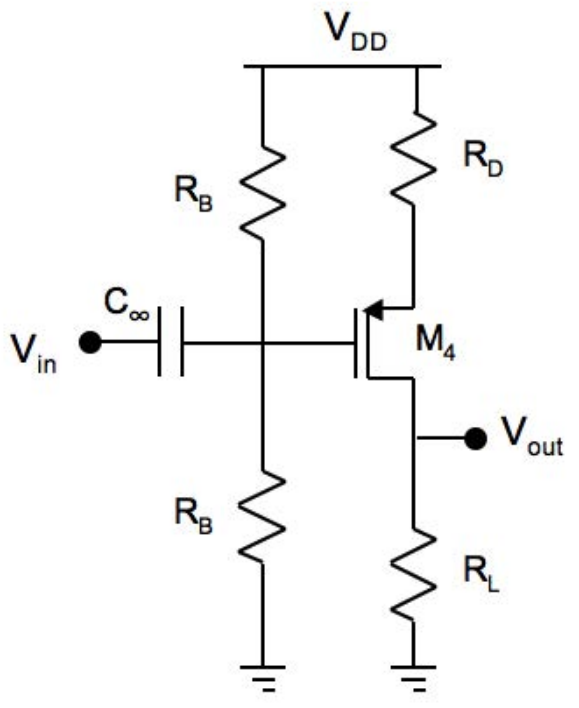
\includegraphics[scale=0.25, center]{p1a.png}\\
    We will let $I_B$ be the bias current that runs through both $R_D$ and $R_L$.  Then we can define the DC voltages of the gate, source, and drain:
    \begin{align}
        V_G &= V_{DD} \cdot \left(\frac{R_B}{R_B \cdot R_B}\right) = \frac{V_{DD}}{2} = 2\,V
        \label{eq:gate_v}\\[0.25cm]
        V_D &= I_B \cdot R_L
        \label{eq:drain_v}\\[0.25cm]
        V_S &= V_{DD} - I_B \cdot R_D
        \label{eq:source_v}
    \end{align}
    }
    
    We want to bias the amplifier to be in saturation, so we can substitute \textit{Eq.~\ref{eq:source_v}} and \textit{Eq.~\ref{eq:gate_v}} into the current equation to solve for $R_D$:
    \begin{align*}
        I_B &= \underbrace{\left(\frac{W}{2L}\right)\,k`}_\phi {\left(V_{SG} - V_T\right)}^2\\[0.25cm]
        &= \phi\,{\left(V_S - V_G - V_T\right)}^2\\[0.25cm]
        &= \phi\,{\left(V_{DD} - I_B \cdot R_D - \frac{V_{DD}}{2} - V_T\right)}^2\\[0.25cm]
        &= \phi\,{\left(4\,V I_B \cdot R_D - 2\,V - 1\,V\right)}^2\\[0.25cm]
        &= \phi\,{\left(1\,V - I_B \cdot R_D\right)}^2\\[0.25cm]
        &= \phi\,\left(1\,V - 2(I_B \cdot R_D) + {I_B}^2\,{R_D}^2\right)\\[0.25cm]
        \implies 0 &= \underbrace{\phi\,{I_B}^2}_A {R_D}^2 - \underbrace{2\phi I_B}_B R_D + \underbrace{\phi - I_B}_C
    \end{align*}
    \newpage\noindent
    Plugging into the given parameters of $\phi$ and $2\,mA$ for $I_B$ yields the quadratic equation:
    \begin{equation}
        \num{1.6e-8}\,{R_D}^2 - \num{1.6e-5}\,R_D + 0.002 = 0
    \end{equation}
    
    There are two solutions to the above equation:
    \begin{align*}
        R_{D_1} &= 853.55339059327 \approx 854\,\Omega\\[0.25cm]
        R_{D_2} &= 146.44660940673 \approx 146\,\Omega\\[0.25cm]
    \end{align*}
    
    This gives two possibilities for $V_S$:
    \begin{align*}
        V_{S_1} &= 4\,V - (2\,mA)(854\,\Omega) \approx 2.292\,V\\[0.25cm]
        V_{S_2} &= 4\,V - (2\,mA)(146\,\Omega) \approx 3.708\,V\\[0.25cm]
    \end{align*}

    This gives two possibilities for $V_{SG}$:
    \begin{align*}
        V_{{SG}_1} &= 2.2924\,V - 2\,V \approx 0.292\,V\\[0.25cm]
        V_{{SG}_2} &= 3.708\,V - 2\,V \approx 1.708\,V\\[0.25cm]
    \end{align*}
    
    Since the first result would give us a cut-off condition, we have:
    \begin{align*}
        \Aboxed{R_D &= 146\,\Omega}\\[0.25cm]
        \Aboxed{V_S &= 3.708\,V}\\[0.25cm]
        \Aboxed{V_{SG} &= 1.708\,V}
    \end{align*}
    
    Now we move on to small-signal analysis.  We can directly compute the transconductance using \textit{Eq.~\ref{eq:mos_transconductance}}:
    \begin{align*}
        g_m &= \frac{2 \cdot I_{SD}}{V_{SG} - \left|V_T\right|} = \frac{4\,mA}{1.708\,V - 1\,V}\\[0.25cm]
        &= \frac{4\,mA}{0.708\,V} = 0.0056497175\,S\\[0.25cm]
        \Aboxed{g_m &\approx 5.65\,mS}
    \end{align*}
    \newpage\noindent
    Below is a picture of the small signal model we will use to find an expression for the gain.  In AC analysis, the large capacitor will act as a wire.
    
    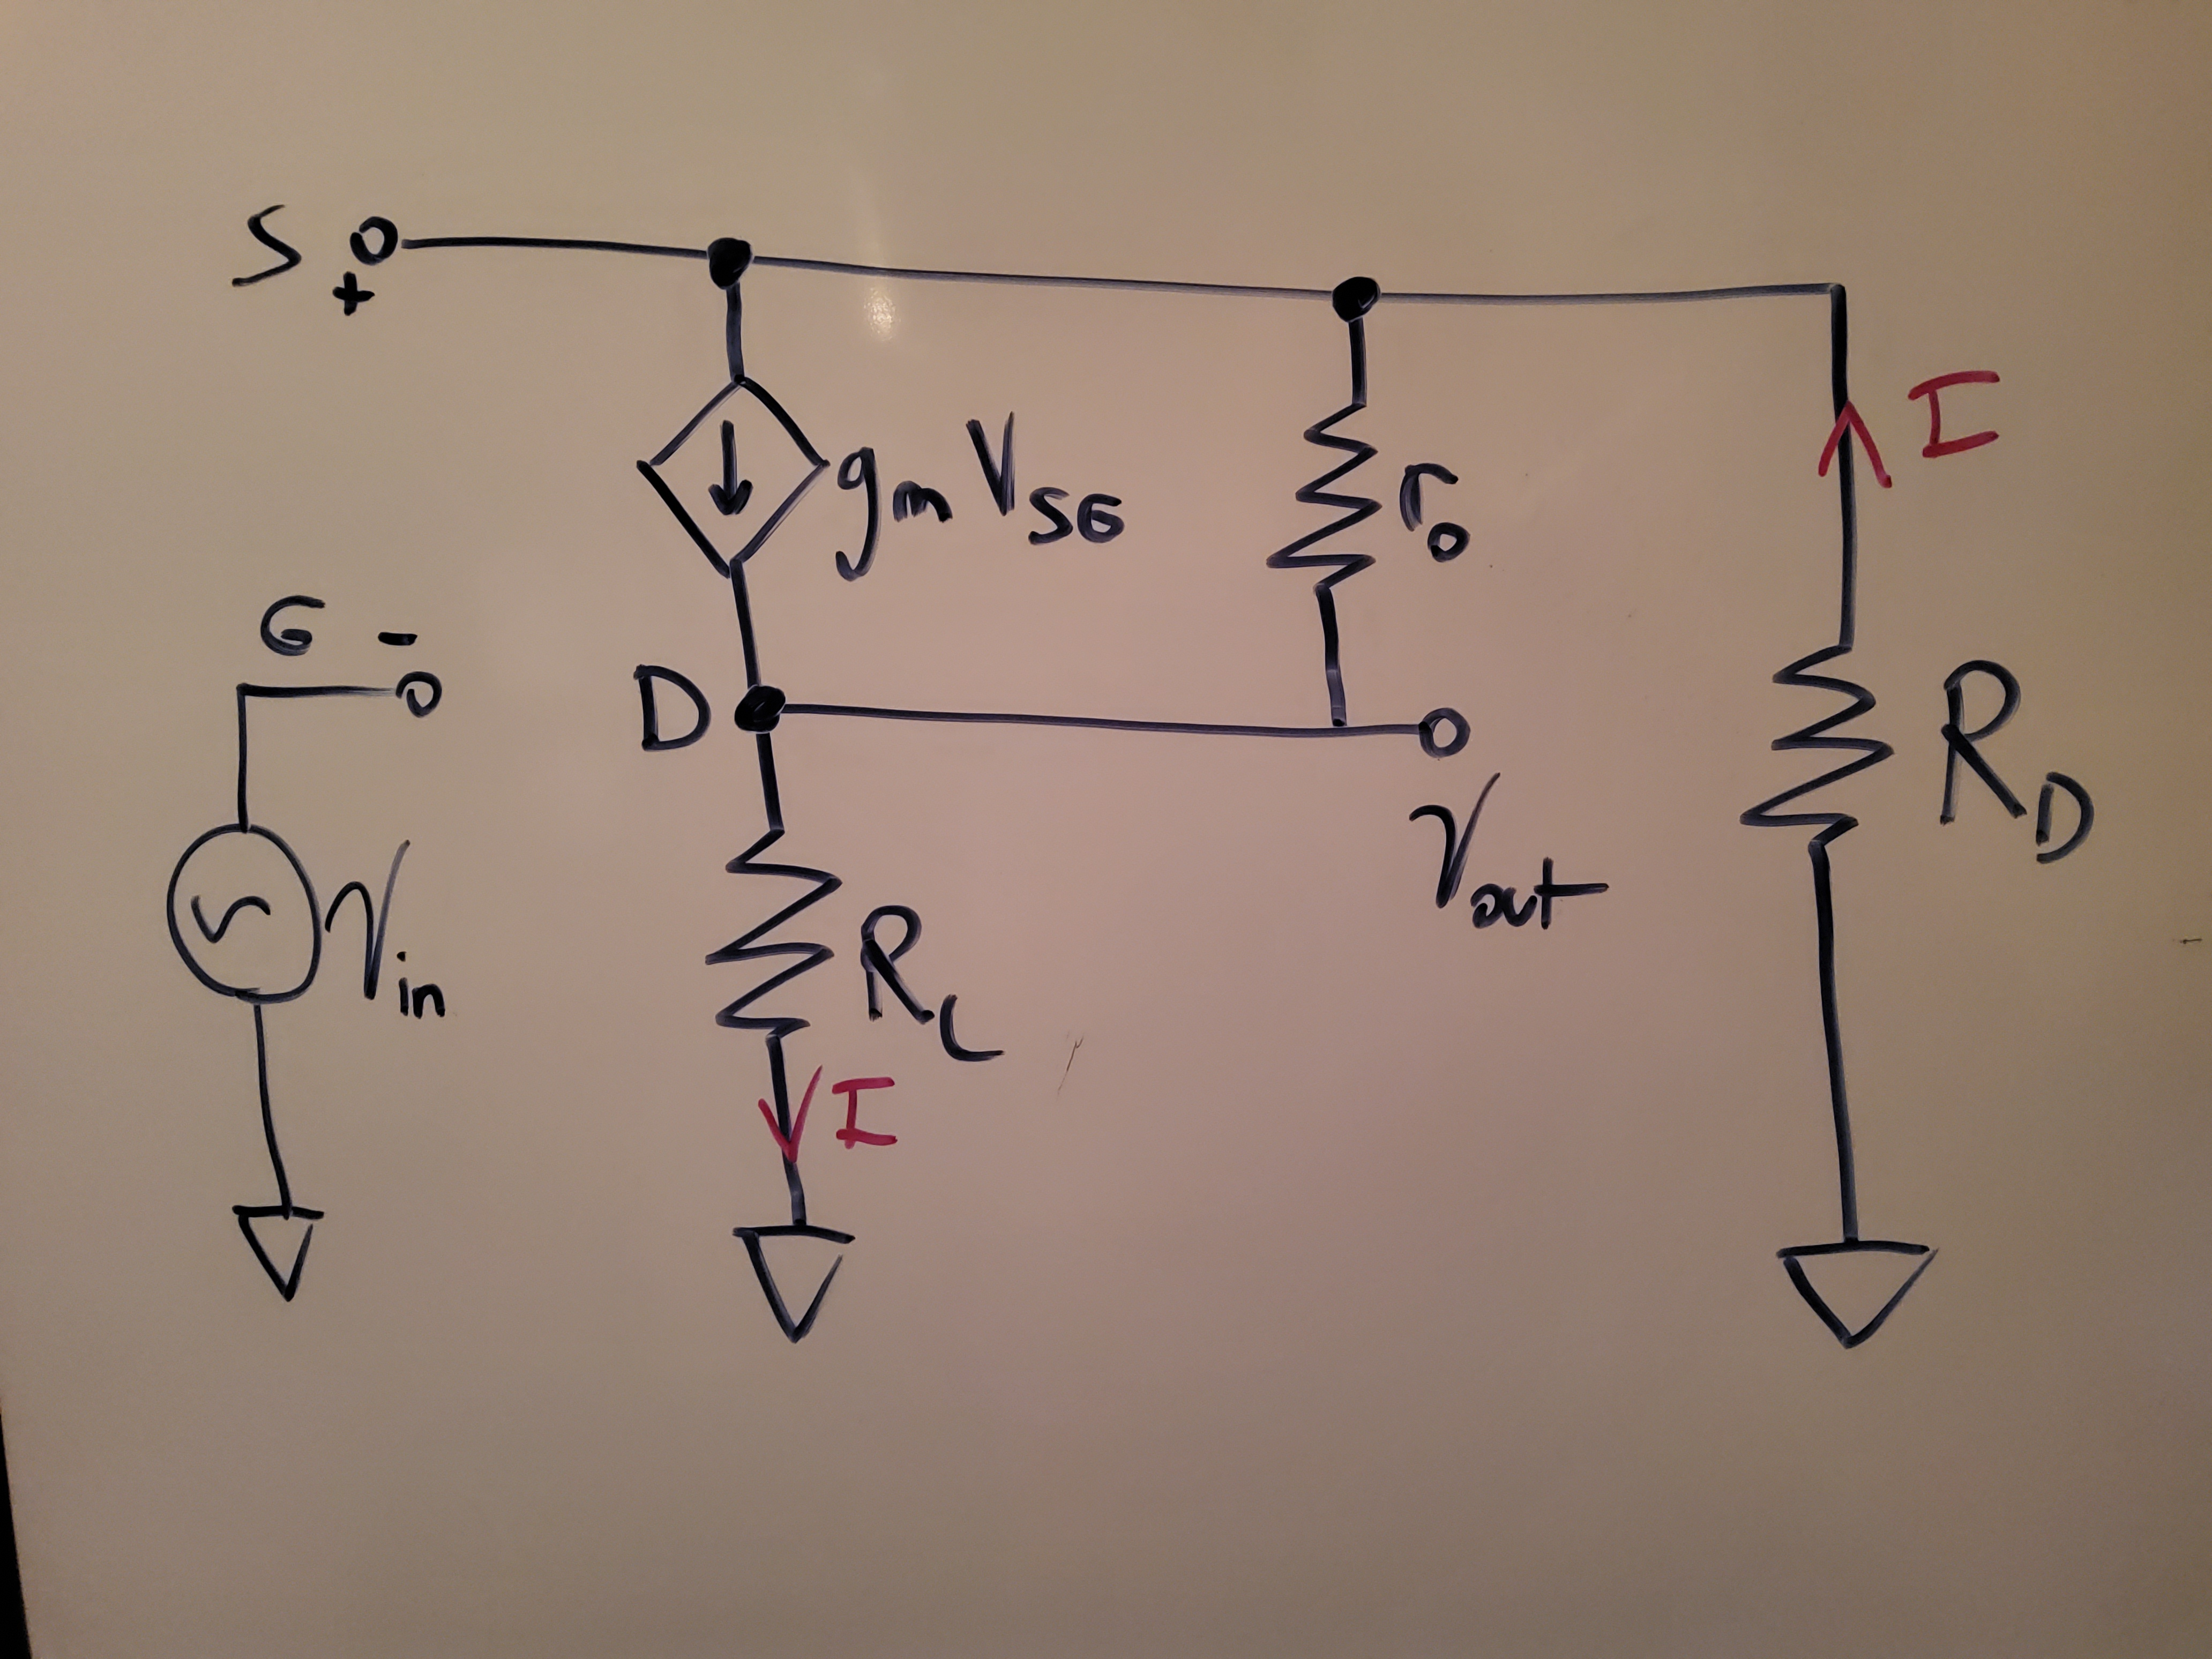
\includegraphics[scale=0.1, center]{p1a.jpg}\\
    
    We define $I$ as the current entering the source through $R_D$, and leaving the drain through $R_L$.  Then we have three equations:
    
    \begin{align}
        I &= g_m\,V_{SG} + \frac{V_{SD}}{r_o}
        \label{eq:i1}\\[0.25cm]
        I &= \frac{-V_S}{R_D}
        \label{eq:i2}\\[0.25cm]
        I &= \frac{V_D}{R_L}
        \label{eq:i3}
    \end{align}
    
    We see that $V_D = v_{out}$ and $V_G = v_{in}$.  Setting \textit{Eq.~\ref{eq:i3}} equal to \textit{Eq.~\ref{eq:i1}}:
    \begin{align*}
        \frac{V_D}{R_L} &= g_m\,V_{SG} + \frac{V_{SD}}{r_o}\\[0.25cm]
        \frac{v_{out}}{R_L} &= g_m\,V_S - g_m\,v_{in} + \frac{V_S}{r_o} - \frac{v_{out}}{r_o}\\[0.25cm]
        \implies v_{out}\left(\frac{1}{r_o} + \frac{1}{R_L}\right) &= -g_m\,v_{in} + V_S\left(g_m + \frac{1}{r_o}\right)
    \end{align*}

    Equating \textit{Eq.~\ref{eq:i2}} to \textit{Eq.~\ref{eq:i3}}:
    \begin{align*}
        \frac{-V_S}{R_D} &= \frac{V_D}{R_L}\\[0.25cm]
        \implies V_S &= -v_{out}\left(\frac{R_D}{R_L}\right)
    \end{align*}
    
    Substituting the above equation:
    \begin{align*}
        v_{out}\left(\frac{1}{r_o} + \frac{1}{R_L}\right) &= -g_m\,v_{in} + -v_{out}\left(\frac{R_D}{R_L}\right)\left(g_m + \frac{1}{r_o}\right)\\[0.25cm]
        \implies &v_{out}\left[\left(\frac{1}{r_o} + \frac{1}{R_L}\right) + \left(\frac{R_D}{R_L}\right)\left(g_m + \frac{1}{r_o}\right)\right] = -g_m\,v_{in}\\[0.25cm]
        \implies &\frac{v_{out}}{v_{in}} = -\left[\frac{g_m}{\left(\frac{r_o + R_L}{r_o\,R_L}\right)+ \left(\frac{R_D}{R_L}\right)\left(\frac{1 + g_m\,r_o}{r_o}\right)}\right]
    \end{align*}

    Our final expression for the gain:
    \begin{equation}
        \boxed{A_v = \frac{v_{out}}{v_{in}} = -\left[\frac{g_m\,r_o\,R_L}{\left(r_o + R_L\right)+ R_D \left(1 + g_m\,r_o\right)}\right]}
        \label{eq:circ_gain}
    \end{equation}
    
    Now that we have an expression for the gain, we can plug in all known values to solve for $R_L$:
    \begin{align*}
        -5 = - \left(\frac{283.5\,R_L}{(R_L + 50\,k) + 41535}\right)\\[0.25cm]
        \implies -457675 - 5\,R_L = -283.5\,R_L\\[0.25cm]
        \implies 278.5\,R_L = 457675\\[0.25cm]
        \implies \Aboxed{R_L \approx 1643\,\Omega}
    \end{align*}
    
    With $R_L$ we now have that $V_D = I_B \cdot R_L = (2\,mA)(1643\,\Omega) = 3.286\,V$.  This gives us that $V_{SG} = 3.708\,V - 3.286\,V = -0.422\,V \not> V_{OV} = V_{SG} - \left|V_T\right| = 0.708\,V$.
    
    \vspace{0.5cm}
    Thus, the problem with this amplifier is that there is no way to bias it so that it operates in the saturation region.
    \newpage\noindent
    %%%%%%%%%%%%%%%%%%
    %%% SOLUTION B %%%
    %%%%%%%%%%%%%%%%%%
    \item
    {
    Below is the given circuit:\\
    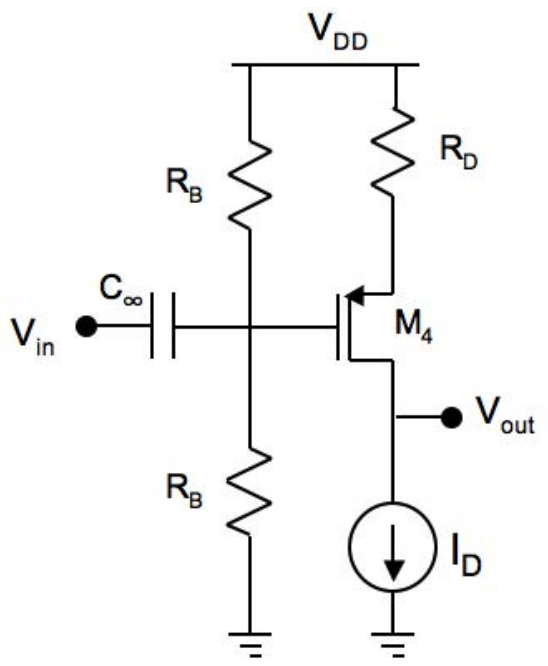
\includegraphics[scale=0.35, center]{p1b.png}\\
    }
    The method we used to find $R_D$ in part (\textit{a}) will not change due to the new topology, thus its value is still $146\,\Omega$, and the current source still biases the saturation current to $2\,mA$.  $V_D$ must be $0.2\,V$ for the required headroom.  Then we have:
    \begin{align*}
        V_{SD} &= V_{DD} - I_D \cdot R_D - V_D\\[0.25cm]
        &= 4\,V -2\,mA \cdot 146\,\Omega - 0.2\,V\\[0.25cm]
        &= 3.508\,V > V_{SG} - \left|V_T\right| = 0.708\,V
    \end{align*}

    We see that this topology will work for saturation.  Now we want to find the new gain expression.  Because we have replaced $R_L$ with an ideal current source, we will take the limit of \textit{Eq.~\ref{eq:circ_gain}} as the resistance of $R_L$ becomes infinite:
    \begin{align*}
        \lim_{R_L\to\infty} &-\left[\frac{g_m\,r_o\,R_L}{\left(r_o + R_L\right)+ R_D \left(1 + g_m\,r_o\right)}\right]\\[0.25cm]
        &= -\left[\frac{g_m\,r_o\,\infty}{\left(r_o + \infty\right)+ R_D \left(1 + g_m\,r_o\right)}\right]
        &\textit{$R_D \left(1 + g_m\,r_o\right) \ll \infty \gg r_o$}\\[0.25cm]
        &= -\left[\frac{\cancel{\infty}(g_m\,r_o)}{\cancel{\infty}}\right]\\[0.25cm]
        \Aboxed{&= -g_m\,r_o}
    \end{align*}
    Plugging in values for $g_m$ and $r_o$ gives a gain of $\boxed{\approx -282.5}$.  The problem is fixed in that we can bias this amplifier to have a large gain, and be in saturation.  This is because the voltage drop at the source is no longer proportional to $R_L$, which results in the proper headroom to bias the amplifier in the desired operating region. 
    \newpage\noindent
    %%%%%%%%%%%%%%%%%%
    %%% SOLUTION C %%%
    %%%%%%%%%%%%%%%%%%
    \item
    {
    Below is the given circuit:\\
    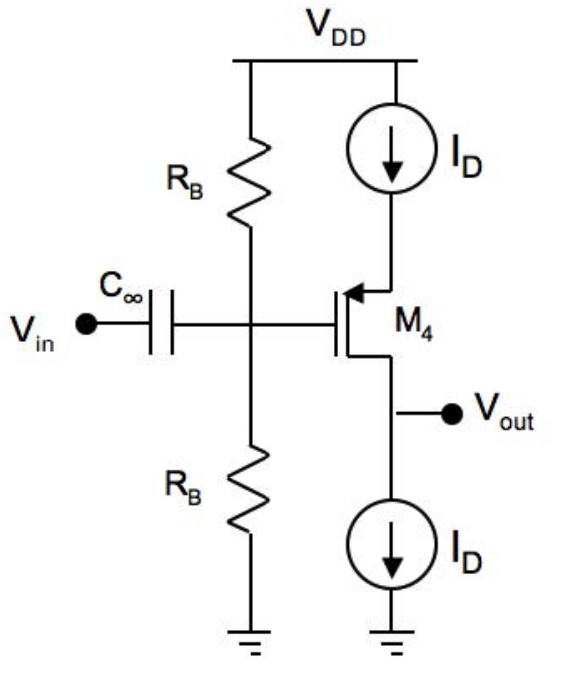
\includegraphics[scale=0.35, center]{p1c.png}\\
    Now that we have replaced both $R_L$ and $R_D$ with ideal current sources, we will take the limit of both \textit{Eq.~\ref{eq:circ_gain}} as their resistances become infinite:
    \begin{align*}
        \lim_{R_L,\;R_D\to\infty} &-\left[\frac{g_m\,r_o\,R_L}{\left(r_o + R_L\right)+ R_D \left(1 + g_m\,r_o\right)}\right]\\[0.25cm]
        &= -\left[\frac{g_m\,r_o\,\infty}{\infty\ + \infty \left(1 + g_m\,r_o\right)}\right]\\[0.25cm]
        &= -\left[\frac{\cancel{\infty}(g_m\,r_o)}{\cancel{\infty}\left(1 + 1 + g_m\,r_o\right)}\right]\\[0.25cm]
        \Aboxed{&= -\left(\frac{g_m\,r_o}{2 + g_m\,r_o}\right)}
    \end{align*}
    }
    
    By inspection this expression for the gain is just slightly less than 1.  We can also analyze the gain from the perspective of the small-signal model, in which the current sources become open circuits.  In this case there is infinite output resistance, but with zero voltage at the output, which implies a gain of 0.
\end{enumerate}
%%%%%%%%%%%%%%%%%%%%%%%%%%%%%%%%%%%%%%%%%%%%%%%%%%%%%%%%%%%%%%%%%%%%%%%%%%%%%%%%%%%%%%%%%%%%%%%%%%%%%%%%%%%
%                                           QUESTION 2                                                    %
%%%%%%%%%%%%%%%%%%%%%%%%%%%%%%%%%%%%%%%%%%%%%%%%%%%%%%%%%%%%%%%%%%%%%%%%%%%%%%%%%%%%%%%%%%%%%%%%%%%%%%%%%%%
\newpage
\section{1T Amplifiers Practice}
\textbf{\emph{Given: }} Different single-transistor circuit topologies.

\vspace{0.5cm}
\noindent
\textbf{\emph{Find: }} \textit{Parts (a-c):  }For each of the following circuits, please derive the equivalent two-port model, including circuit $G_m$ and Thevenin resistances. You may assume all FETs are biased in saturation. Do not omit the effect of channel length modulation. Assume an input source resistance of $R_{in}$ for all inputs, and open circuit for all outputs.

\vspace{0.5cm}
\noindent
\textit{Part (d)}  In applications such as photonic links, it’s common that the input has a finite resistance with a weak current signal that we’d like to capture and amplify. Furthermore the output of our circuit may need to drive large capacitive loads at fairly high speeds. For this reason, it may be necessary to use multiple stages to satisfy all the requirements of the application. Such
circuits may become convoluted very fast, and impossible to analyze using KCL/KVL. For the following multiple stage amplifier circuit, use the two port models that you’ve derived to compute the circuit’s gain, $v_{out}/i_{in}$.  Draw the cascaded two port diagrams to show your work. Assume that $C_{ac}$ is large and all the transistors are in saturation. The transconductances, backgate transconductances and output resistances of $M_1$ , $M_2$ and $M_3$ are $g_{m_1}$, $g_{m_2}$, $g_{m_3}$, $g_{{mb}_1}$, $g_{{mb}_2}$, $g_{{mb}_3}$, and $r_{o_1}$, $r_{o_2}$, $r_{o_3}$ respectively. You can leave your answer in terms of $R_{in}$, $R_{out}$, and $G_m$ of the stages (where the two port parameters of the first stage is e.g. $R_{{in}_1}$, $R_{{out}_1}$, and $G_{m_1}$).

\newpage
\noindent
\textbf{\emph{Solution: }}

\begin{enumerate}[label=(\alph*)]
    %%%%%%%%%%%%%%%%%%
    %%% SOLUTION A %%%
    %%%%%%%%%%%%%%%%%%
    \item
    {
    Below is the given circuit:
    
    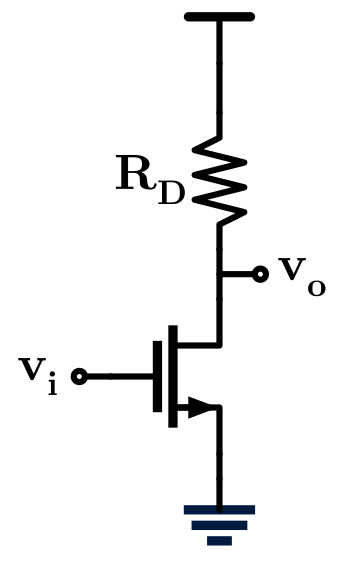
\includegraphics[scale=0.25, center]{p2a.png}\\
    Below is the two-port model we wish to derive, and the small-signal models that will be used for analysis; including the body effect.
    
    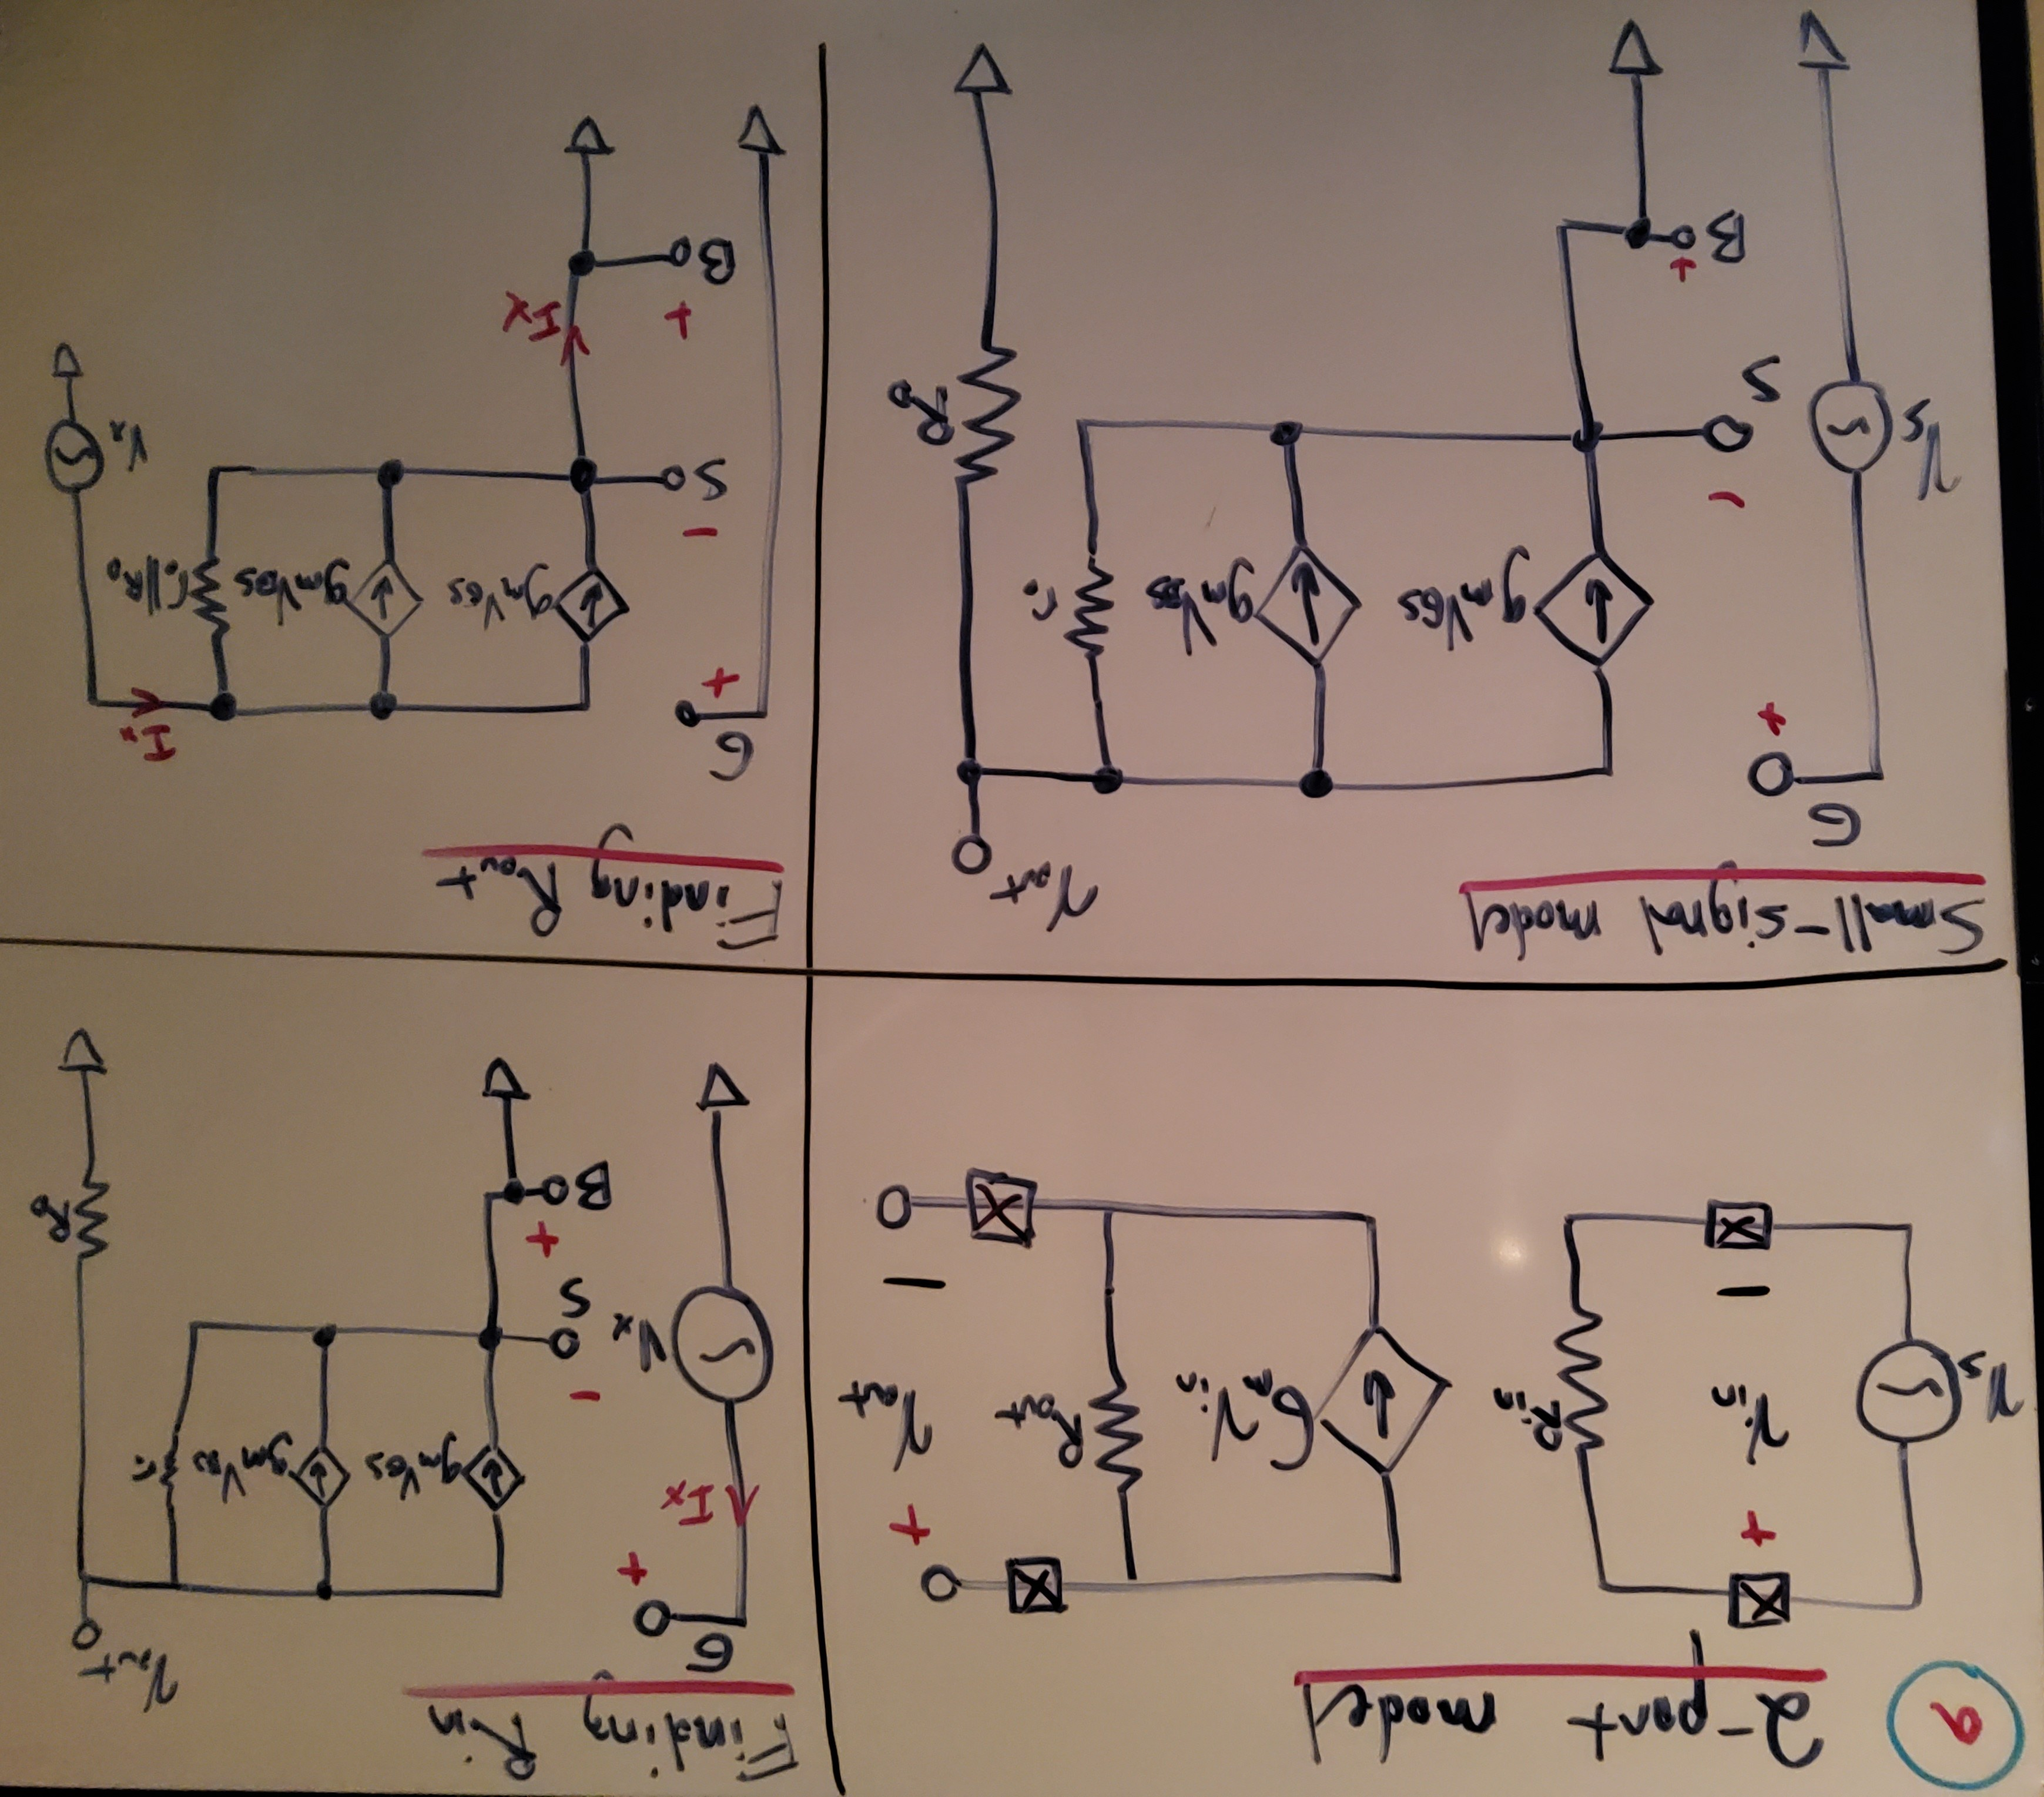
\includegraphics[scale=0.1, center, angle = 180]{p2a.jpg}\\
    \newpage
    \underline{\textbf{Finding $R_{in}$}}\\[0.25cm]
    In the picture it is obvious that the current from our test source sees an infinite input resistance at the gate.
    
    $\therefore\qquad\boxed{R_{{in}_A} = \infty}$
    \vspace{0.5cm}
    
    \underline{\textbf{Finding $R_{out}$}}\\[0.25cm]
    Noting that $V_G = V_S = V_B = 0\,V$, the current from our test source is :
    \begin{align}
        I_X &= \frac{V_{DS}}{r_o \parallel R_D} + \cancelto{0}{g_m\,V_{GS}} + \cancelto{0}{g_m\,V_{BS}}\\[0.25cm]
        &= \frac{V_X}{r_o \parallel R_D}\\[0.25cm]
        \implies \Aboxed{R_{{out}_A} &= \frac{V_X}{I_X} = r_o \parallel R_D}
    \end{align}
    
    \underline{\textbf{Finding $G_m$}}\\[0.25cm]
    We can equate the two-port model short circuit current at the output to the small-signal model short circuit current at the output to find $G_m$.
    
    The two-port model short circuit current at the output can be seen by inspection, and it is $I_{SC} = G_m\,v_{in}$.
    
    The small-signal model short circuit current at the output is:
    \begin{align}
        i_{sc} &= g_m\,V_{GS} + \cancelto{0}{g_m\,V_{BS}}\\[0.25cm]
        &= g_m\,v_s
    \end{align}
    
    Noting that $v_{in} = v_s$, and equating $I_{SC}$ to $i_{sc}$:
    \begin{align}
        G_m\,v_s &= g_m\,v_s\\[0.25cm]
        \implies\Aboxed{G_{m_A} &= g_m}
    \end{align}
    }
    \newpage
    %%%%%%%%%%%%%%%%%%
    %%% SOLUTION B %%%
    %%%%%%%%%%%%%%%%%%
    \item
    {
    Below is the given circuit:
    
    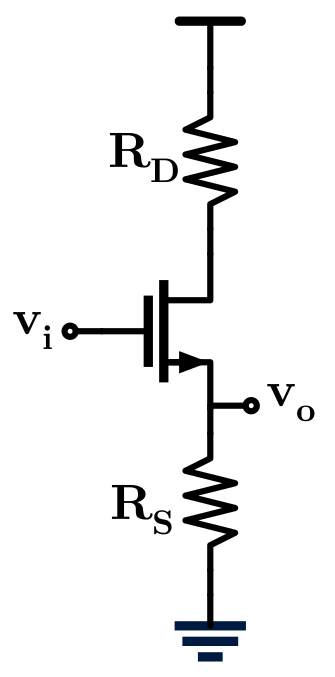
\includegraphics[scale=0.25, center]{p2b.png}\\
    Below is the two-port model we wish to derive, and the small-signal models that will be used for analysis; including the body effect.
    
    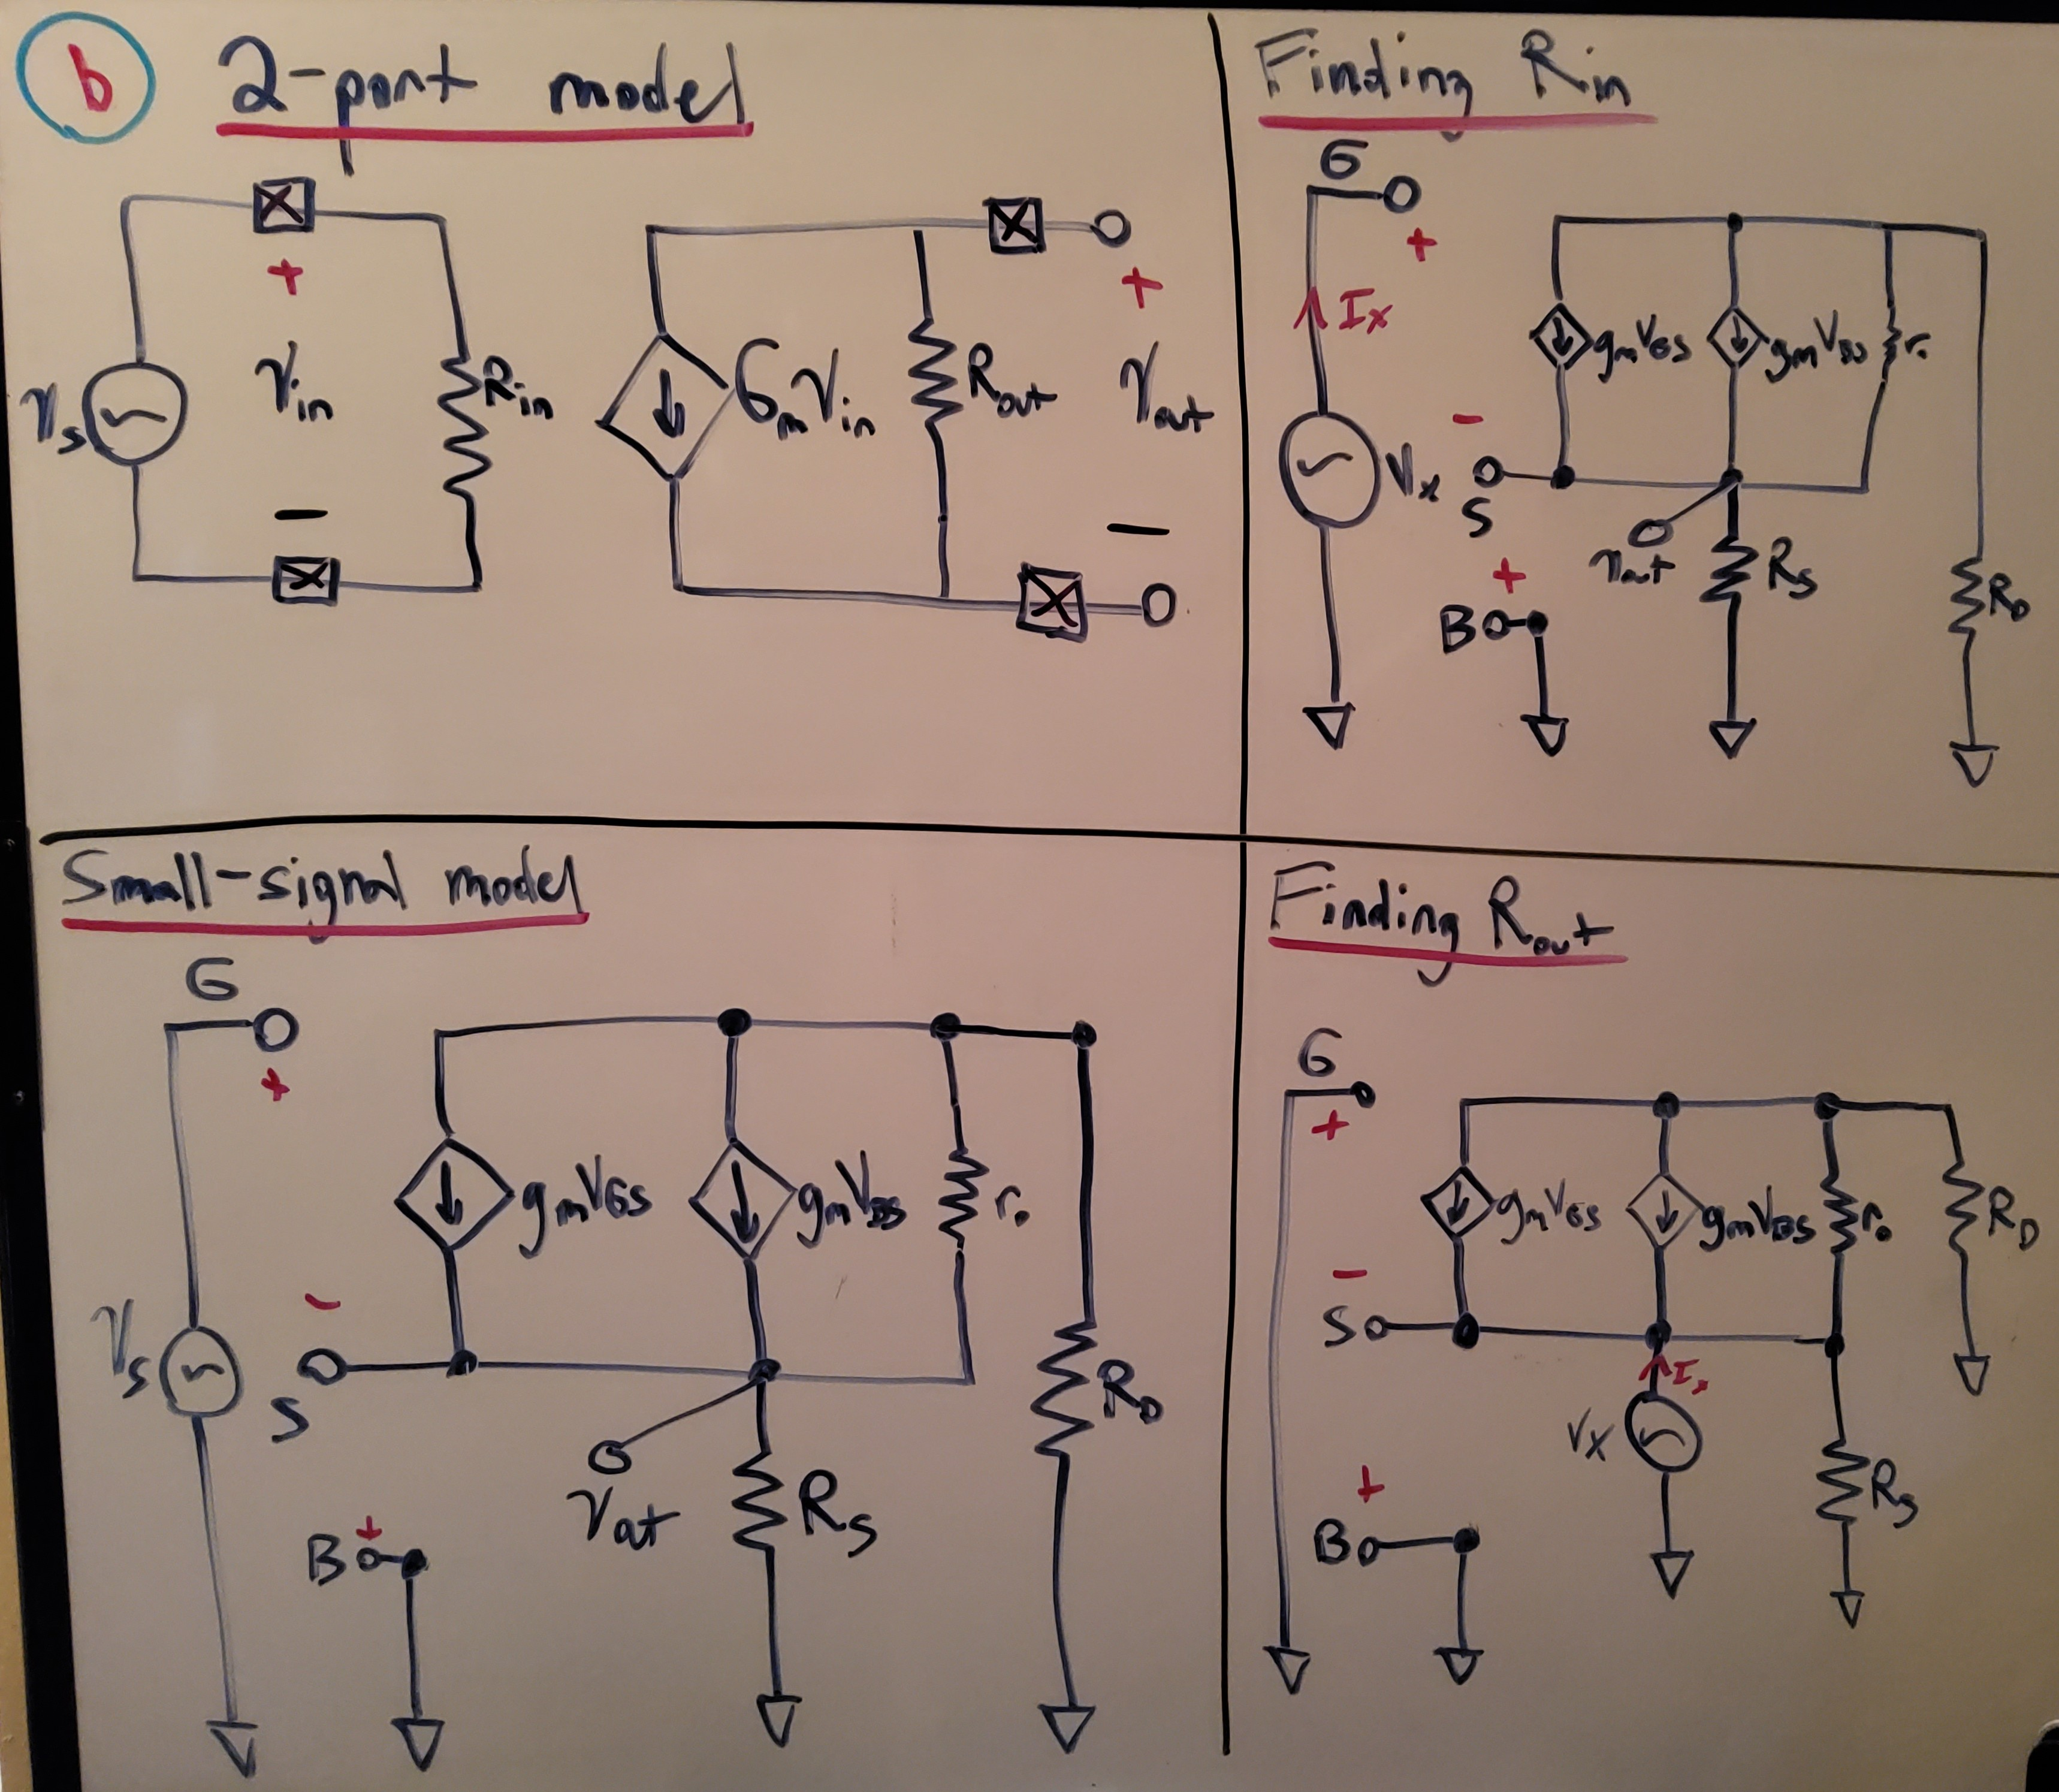
\includegraphics[scale=0.1, center]{p2b.jpg}\\
    \newpage
    \underline{\textbf{Finding $R_{in}$}}\\[0.25cm]
    In the picture it is obvious that the current from our test source sees an infinite input resistance at the gate.
    
    $\therefore\qquad\boxed{R_{{in}_B} = \infty}$
    \vspace{0.5cm}
    
    \underline{\textbf{Finding $R_{out}$}}\\[0.25cm]
    The current from our test source is :
    \begin{align}
        I_X &= \frac{V_S}{R_S} + \frac{V_{SD}}{r_o} - g_m\,V_{GS} - g_m\,V_{BS}\\[0.25cm]
        &= \frac{V_X}{R_S} + \frac{V_X}{r_o} - \frac{V_D}{r_o} + g_m\,V_X + g_{mb}\,V_X\\[0.25cm]
        \implies I_X &= V_X\left(\frac{1}{R_S} + \frac{1}{r_o} + g_m + g_{mb}\right) - \frac{V_D}{r_o}
        \label{eq:node3}
    \end{align}
    
    KCL at the drain node yields:
    \begin{align}
        0 &= \frac{V_D}{R_D} + \frac{V_{DS}}{r_o} + g_m\,V_{GS} + g_m\,V_{BS}\\[0.25cm]
        &= V_D\left(\frac{1}{R_D} + \frac{1}{r_o}\right) - \frac{V_X}{r_o} - g_m\,V_X - g_{mb}\,V_X\\[0.25cm]
        \implies &\;V_D\left(\frac{1}{R_D} + \frac{1}{r_o}\right) = V_X\left(\frac{1}{r_o} + g_m + g_{mb}\right)\\[0.25cm]
        \implies V_D &= V_X\left(\frac{1}{r_o} + g_m + g_{mb}\right)r_o \parallel R_D
        \label{eq:node4}
    \end{align}
    Substituting \textit{Eq.~\ref{eq:node4}} into \textit{Eq.~\ref{eq:node3}}.
    \begin{align*}
        I_X &= V_X\left(\frac{1}{R_S} + \frac{1}{r_o} + g_m + g_{mb}\right) - \frac{V_X\left(\frac{1}{r_o} + g_m + g_{mb}\right)r_o \parallel R_D}{r_o}\\[0.25cm]
        &= V_X\left[\frac{r_o + R_S + r_o R_S g_m + r_o R_S  g_{mb}}{r_o\,R_S}\right]
            - \frac{V_X}{r_o}\left[\left(\frac{1 + g_m r_o + g_{mb} r_o}{r_o}\right)\left(\frac{r_o\,R_D}{r_o + R_D}\right)\right]\\[0.25cm]
        &= V_X\left[\frac{r_o + R_S + r_o R_S(g_m + g_{mb})}{r_o\,R_S} - \left(\frac{(1 + g_m r_o + g_{mb} r_o)R_D}{r_o(r_o + R_D)}\right)\right]\\[0.25cm]
        &= V_X\left[\frac{(r_o + R_D)(r_o + R_S + r_o R_S(g_m + g_{mb})) - R_S\,R_D(1 + g_m r_o + g_{mb} r_o)}{r_o\,R_S(r_o + R_D)}\right]
    \end{align*}
    We have arrived at the output resistance for the two-port model:
    \begin{equation}
        \boxed{R_{{out}_B} = \frac{V_X}{I_X} = \left[\frac{r_o\,R_S(r_o + R_D)}{(r_o + R_D)(r_o + R_S + r_o R_S(g_m + g_{mb})) - R_S\,R_D(1 + g_m r_o + g_{mb} r_o)}\right]}
    \end{equation}
    \underline{\textbf{Finding $G_m$}}\\[0.25cm]
    We can equate the two-port model short circuit current at the output to the small-signal model short circuit current at the output to find $G_m$.
    
    The two-port model short circuit current at the output can be seen by inspection, and it is $I_{SC} = G_m\,v_{in}$.
    
    The small-signal model short circuit current across $R_D$ is:
    \begin{align}
        i_{sc} &= -\frac{V_D}{R_D}\\[0.25cm]
        \implies V_D &= i_{sc} \cdot R_D
    \end{align}
    
    With $R_S$ being shorted, the source node is also shorted to ground.  Noting that $V_B = V_S = 0\,V$ and $V_G = v_s$, the small-signal model short circuit current at the output is:
    \begin{align}
        i_{sc} &= -g_m V_{GS} - \cancelto{0}{g_{mb} V_{BS}} \quad + \frac{V_{SD}}{r_o}\\[0.25cm]
        &= g_m v_s - \frac{V_D}{r_o}\\[0.25cm]
        &= g_m v_s - \frac{i_{sc} \cdot R_D}{r_o}\\[0.25cm]
        \implies & i_{sc} \left(1 + R_D\right) = -g_m v_s\\[0.25cm]
        \implies & i_{sc} = -v_s\left(\frac{g_m}{1 + R_D}\right)
    \end{align}

    Noting that $v_{in} = v_s$, and equating $I_{SC}$ to $i_{sc}$:
    \begin{align}
        G_m\,v_s &= -v_s\left(\frac{g_m}{1 + R_D}\right)\\[0.25cm]
        \implies\Aboxed{G_{m_B} &= -\left(\frac{g_m}{1 + R_D}\right)}
    \end{align}
    }
    \newpage
    %%%%%%%%%%%%%%%%%%
    %%% SOLUTION C %%%
    %%%%%%%%%%%%%%%%%%
    \item
    {
    Below is the given circuit:
    
    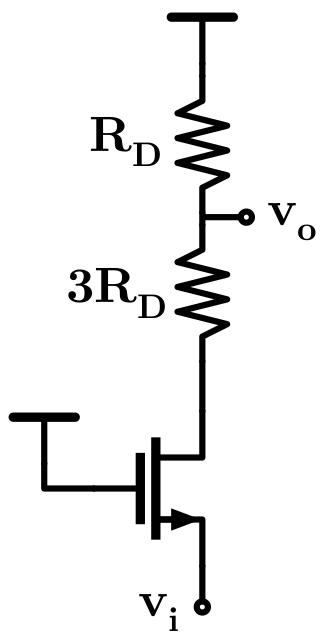
\includegraphics[scale=0.25, center]{p2c.png}\\
    Below is the two-port model we wish to derive, and the small-signal models that will be used for analysis; including the body effect.
    
    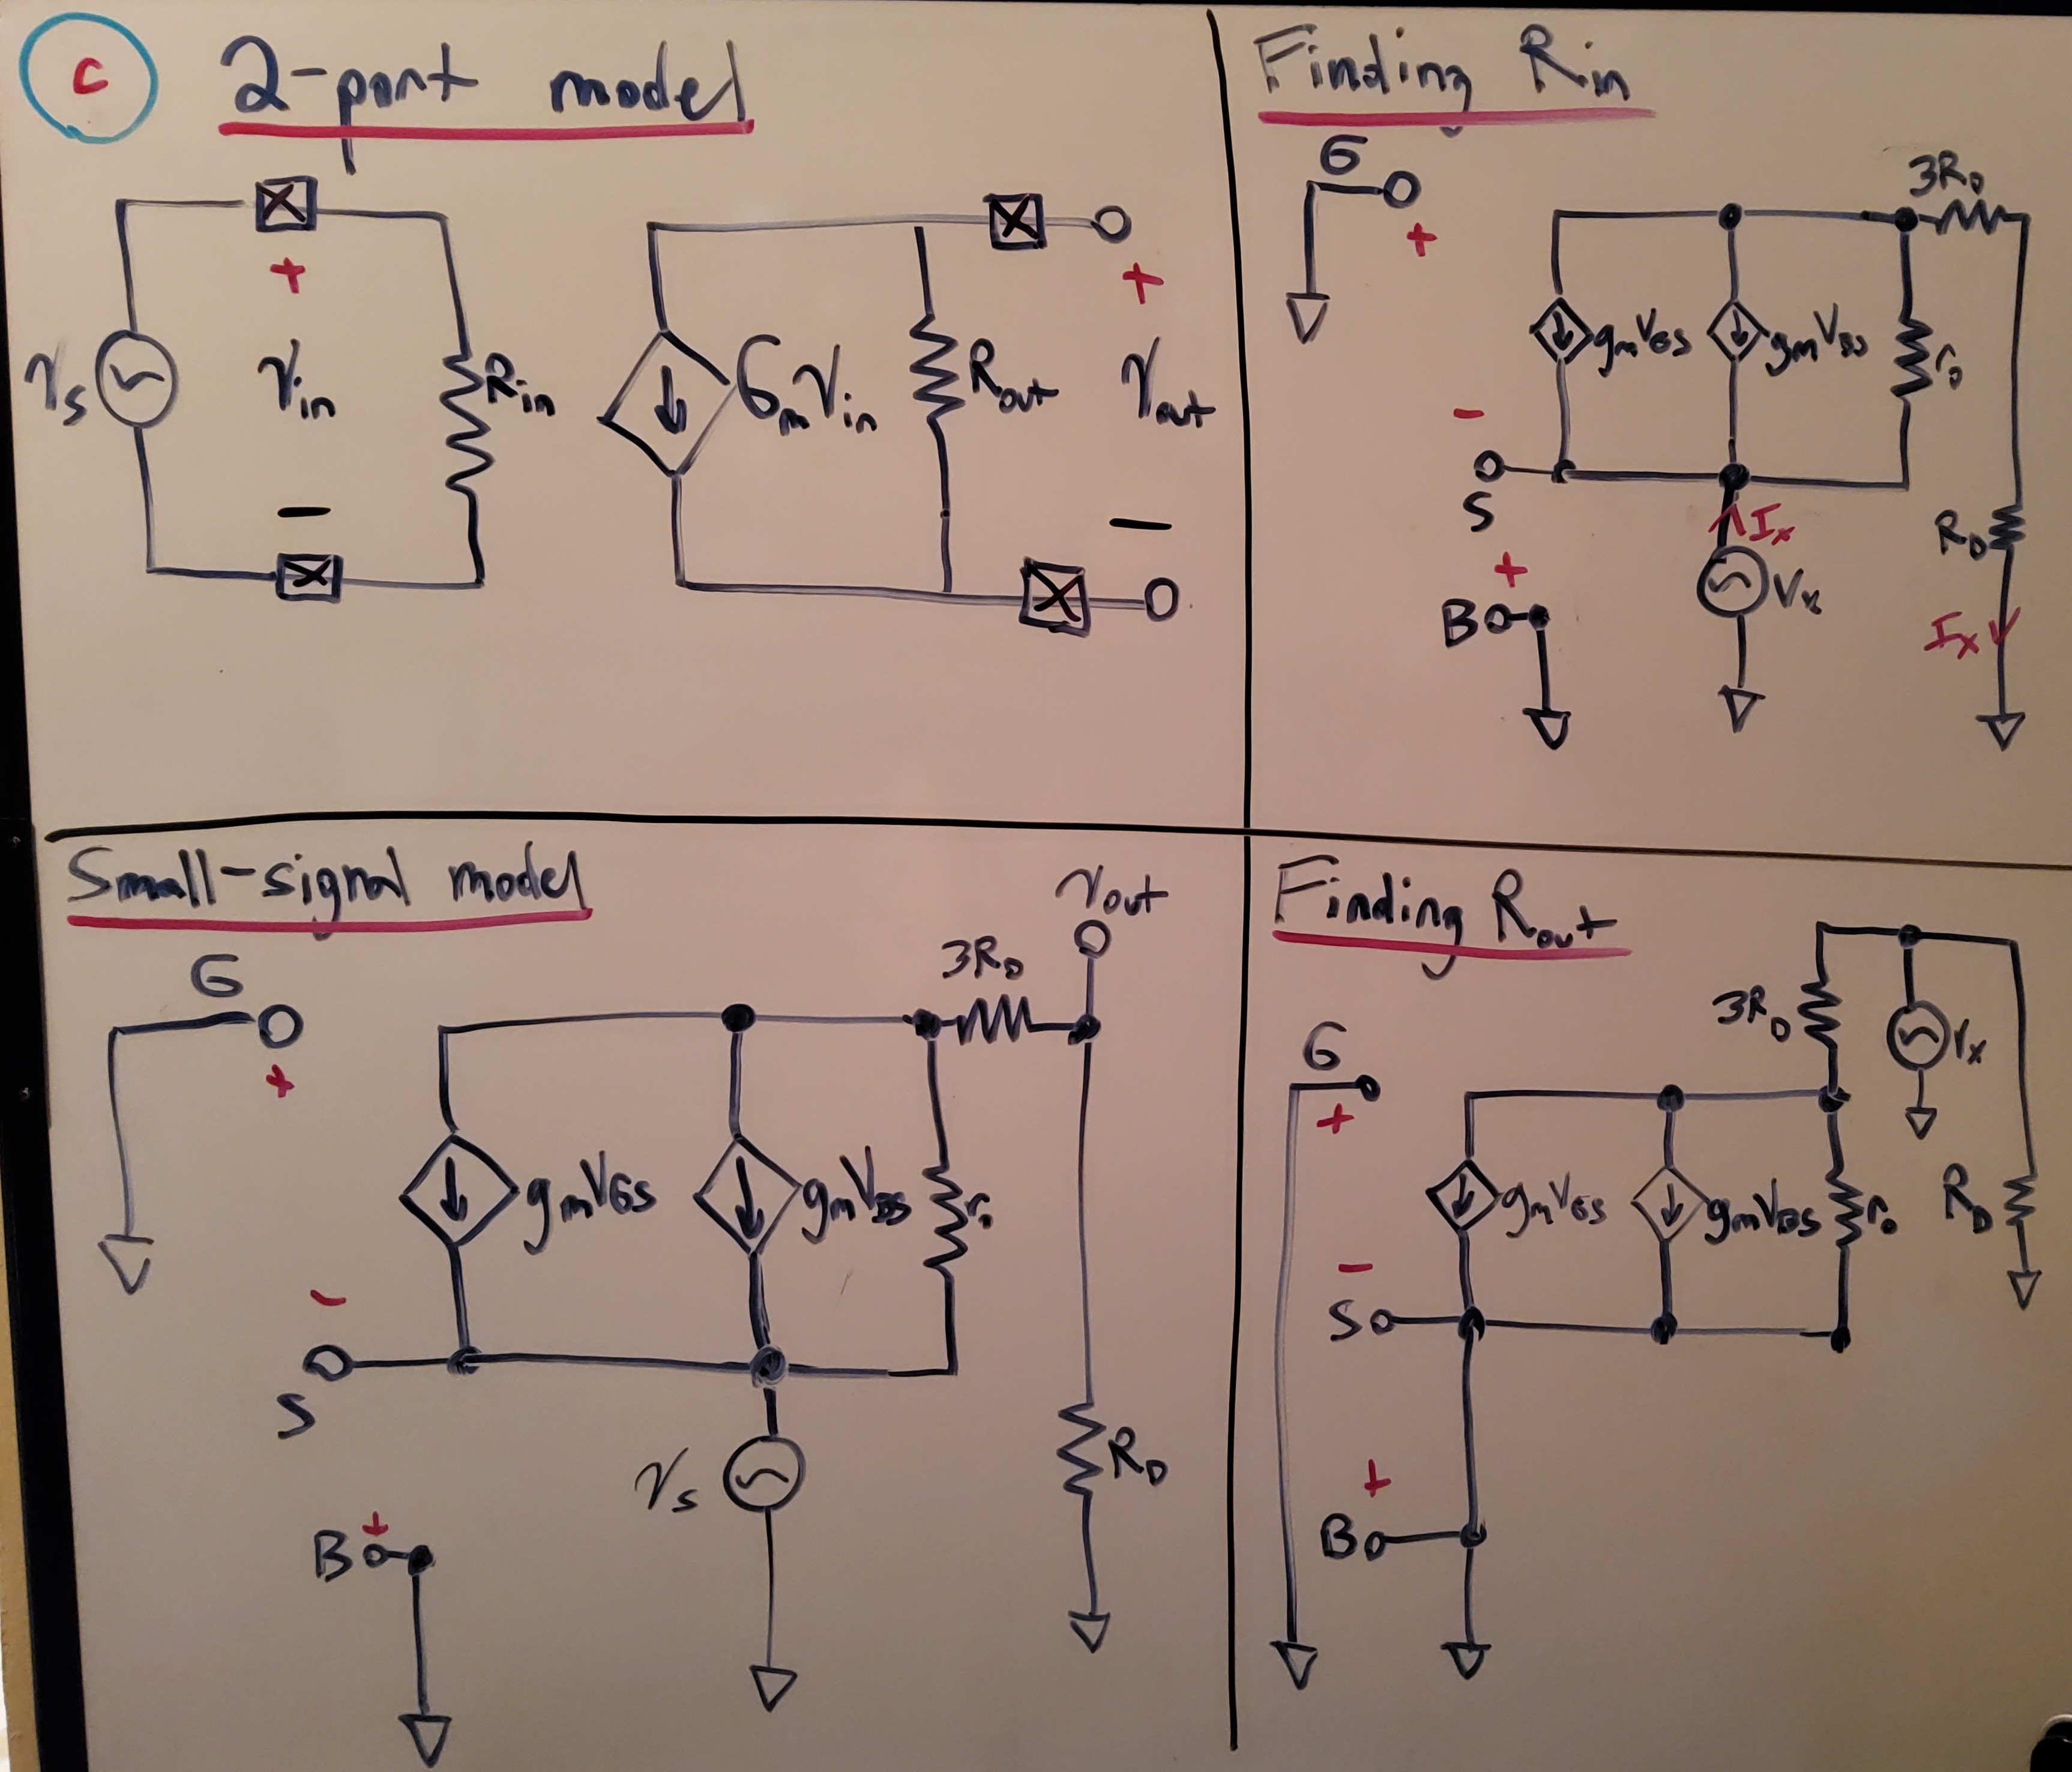
\includegraphics[scale=0.1, center]{p2c.jpg}\\
    \newpage
    \underline{\textbf{Finding $R_{in}$}}\\[0.25cm]
    The current from our test source across the series combination of ${3R}_D$ and $R_D$ is:
    \begin{align}
        I_X &= \frac{V_D}{{4R}_D}\\[0.25cm]
        \implies \Aboxed{V_D &= I_X \cdot {4R}_D}
        \label{eq:node5}
    \end{align}
    Noting that $V_G = V_B = 0\,V$ and $V_S = V_X$, the current from our test source at the source node is :
    \begin{align}
        I_X &= - g_m\,V_{GS} - g_m\,V_{BS} + \frac{V_{SD}}{r_o}\\[0.25cm]
        &= g_m\,V_X + g_{mb}\,V_X + \frac{V_X}{r_o} - \frac{V_D}{r_o}\\[0.25cm]
        \label{eq:node6}
    \end{align}
    Substituting \textit{Eq.~\ref{eq:node5}} into \textit{Eq.~\ref{eq:node6}}.
    \begin{align*}
        I_X &= g_m\,V_X + g_{mb}\,V_X + \frac{V_X}{r_o} - \frac{I_X \cdot {4R}_D}{r_o}\\[0.25cm]
        \implies I_X\left(1 + \frac{{4R}_D}{r_o}\right) &= V_X\left(\frac{1}{r_o} + g_m + g_{mb}\right)\\[0.25cm]
    \end{align*}
    Rearranging, and we have the input resistance:
    \begin{equation}
        \boxed{R_{{in}_C} = \frac{V_X}{I_X} = \frac{r_o + {4R}_D}{1 + g_m r_o + g_{mb} r_o}}
    \end{equation}
    
    \underline{\textbf{Finding $R_{out}$}}\\[0.25cm]
    The current from our test source across the parallel combination of ${3R}_D$ and $R_D$ is:
    \begin{align}
        I_X &= \frac{V_X}{R_D} + \frac{V_X - V_D}{{3R}_D}\\[0.25cm]
        &= \frac{4V_X}{{3R}_D} - \frac{V_D}{{3R}_D} = \frac{4V_X - V_D}{{3R}_D}
        \label{eq:node7}
    \end{align}
    Noting that $V_G = V_B = V_S = 0\,V$, KCL at the drain node yields :
    \begin{align}
        0 &= \frac{V_{DX}}{{3R}_D} + \frac{V_{DS}}{r_o} + \cancelto{0}{g_m V_{GS}} + \cancelto{0}{g_m V_{BS}}\\[0.25cm]
        &= \frac{V_D}{{3R}_D} - \frac{V_X}{{3R}_D} + \frac{V_D}{r_o}\\[0.25cm]
        \implies &= V_D\left(\frac{1}{{3R}_D} + \frac{1}{r_o}\right) = \frac{V_X}{{3R}_D}\\[0.25cm]
        \implies V_D = \frac{V_X}{{3R}_D}\left(r_o \parallel {3R}_D\right)
        \label{eq:node8}
    \end{align}
    Substituting \textit{Eq.~\ref{eq:node8}} into \textit{Eq.~\ref{eq:node7}}.
    \begin{align*}
        I_X &= \frac{4V_X - \frac{V_X}{{3R}_D}\left(r_o \parallel {3R}_D\right)}{{3R}_D}\\[0.25cm]
        &= 4V_X - \left(\frac{\frac{V_X r_o \cancel{{3R}_D}}{\cancel{{3R}_D}(r_o + {3R}_D)}}{{3R}_D}\right)\\[0.25cm]
        &= V_X\left(\frac{4 - \frac{r_o}{r_o + {3R}_D)}}{{3R}_D}\right)\\[0.25cm]
        &= V_X\left(\frac{3r_o + {12R}_D)}{{3R}_D(r_o + {3R}_D)}\right)\\[0.25cm]
    \end{align*}
    Rearranging and simplifying, and we have the output resistance:
    \begin{equation}
        \boxed{R_{{out}_C} = \frac{V_X}{I_X} = \frac{R_D(r_o + {3R}_D)}{r_o + {4R}_D}}
    \end{equation}
    
    \underline{\textbf{Finding $G_m$}}\\[0.25cm]
    We can equate the two-port model short circuit current at the output to the small-signal model short circuit current at the output to find $G_m$.
    
    The two-port model short circuit current at the output can be seen by inspection, and it is $I_{SC} = G_m\,v_{in}$.
    
    The small-signal model short circuit current at the output is:
    \begin{align}
        i_{sc} &= -\frac{V_D}{3R_D}\\[0.25cm]
        \implies V_D &= -i_{sc} \cdot 3R_D
    \end{align}
    
    Noting that $V_B = V_G = 0\,V$ and $V_S = v_s$, the small-signal model short circuit current at the input is:
    \begin{align}
        -i_{sc} &= -g_m V_{GS} - g_{mb} V_{BS} + \frac{V_{SD}}{r_o}\\[0.25cm]
        &= g_m V_{GS} + g_{mb} V_{BS} - \frac{V_{SD}}{r_o}\\[0.25cm]
        &= -g_m v_s - g_{mb} v_s - \frac{v_s}{r_o} + \frac{V_D}{r_o}\\[0.25cm]
        &= -g_m v_s - g_{mb} v_s - \frac{v_s}{r_o} + \frac{-i_{sc} \cdot 3R_D}{r_o}\\[0.25cm]
        \implies & i_{sc} \left(1 + \frac{3R_D}{r_o}\right) = -v_s\left(g_m + g_{mb} + \frac{1}{r_o}\right)\\[0.25cm]
        \implies & i_{sc} = -v_s\left(\frac{1 + g_m r_o + g_{mb} r_o}{r_o + 3R_D}\right)
    \end{align}

    Noting that $v_{in} = v_s$, and equating $I_{SC}$ to $i_{sc}$:
    \begin{align}
        G_m\,v_s &= -v_s\left(\frac{1 + g_m r_o + g_{mb} r_o}{r_o + 3R_D}\right)\\[0.25cm]
        \implies\Aboxed{G_{m_C} &= -\left(\frac{1 + g_m r_o + g_{mb} r_o}{r_o + 3R_D}\right)}
    \end{align}
    }
    \newpage
    %%%%%%%%%%%%%%%%%%
    %%% SOLUTION D %%%
    %%%%%%%%%%%%%%%%%%
    \item
    {
    Below is the given circuit:
    
    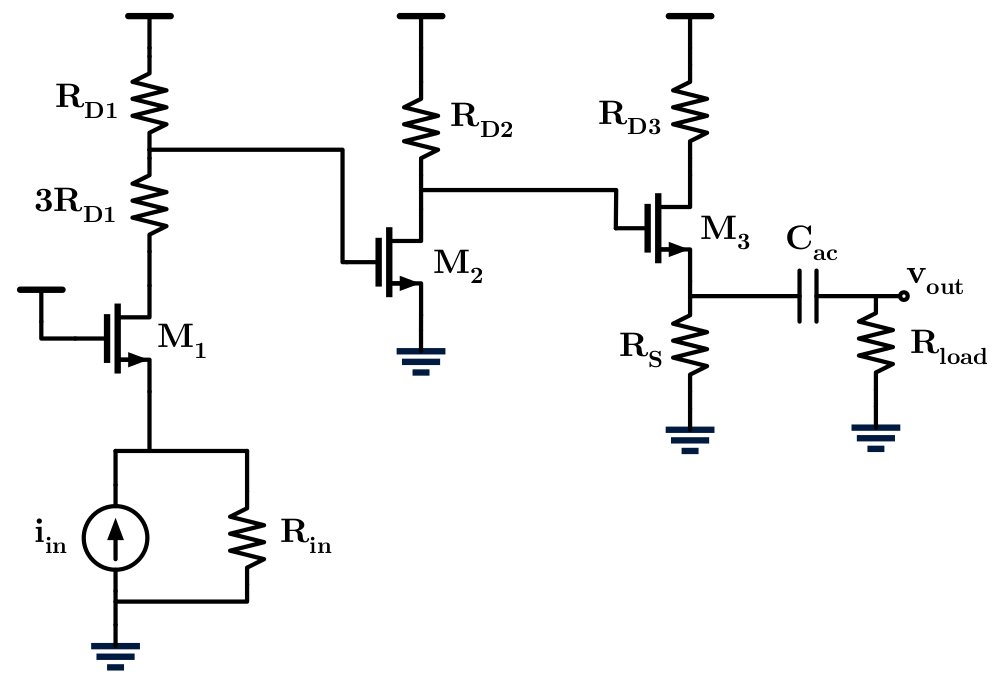
\includegraphics[scale=0.45, center]{p2d.png}\\

    Below is a schematic of the transformed circuit using the two-port models we derived in parts (\textit{a - c}):
    
    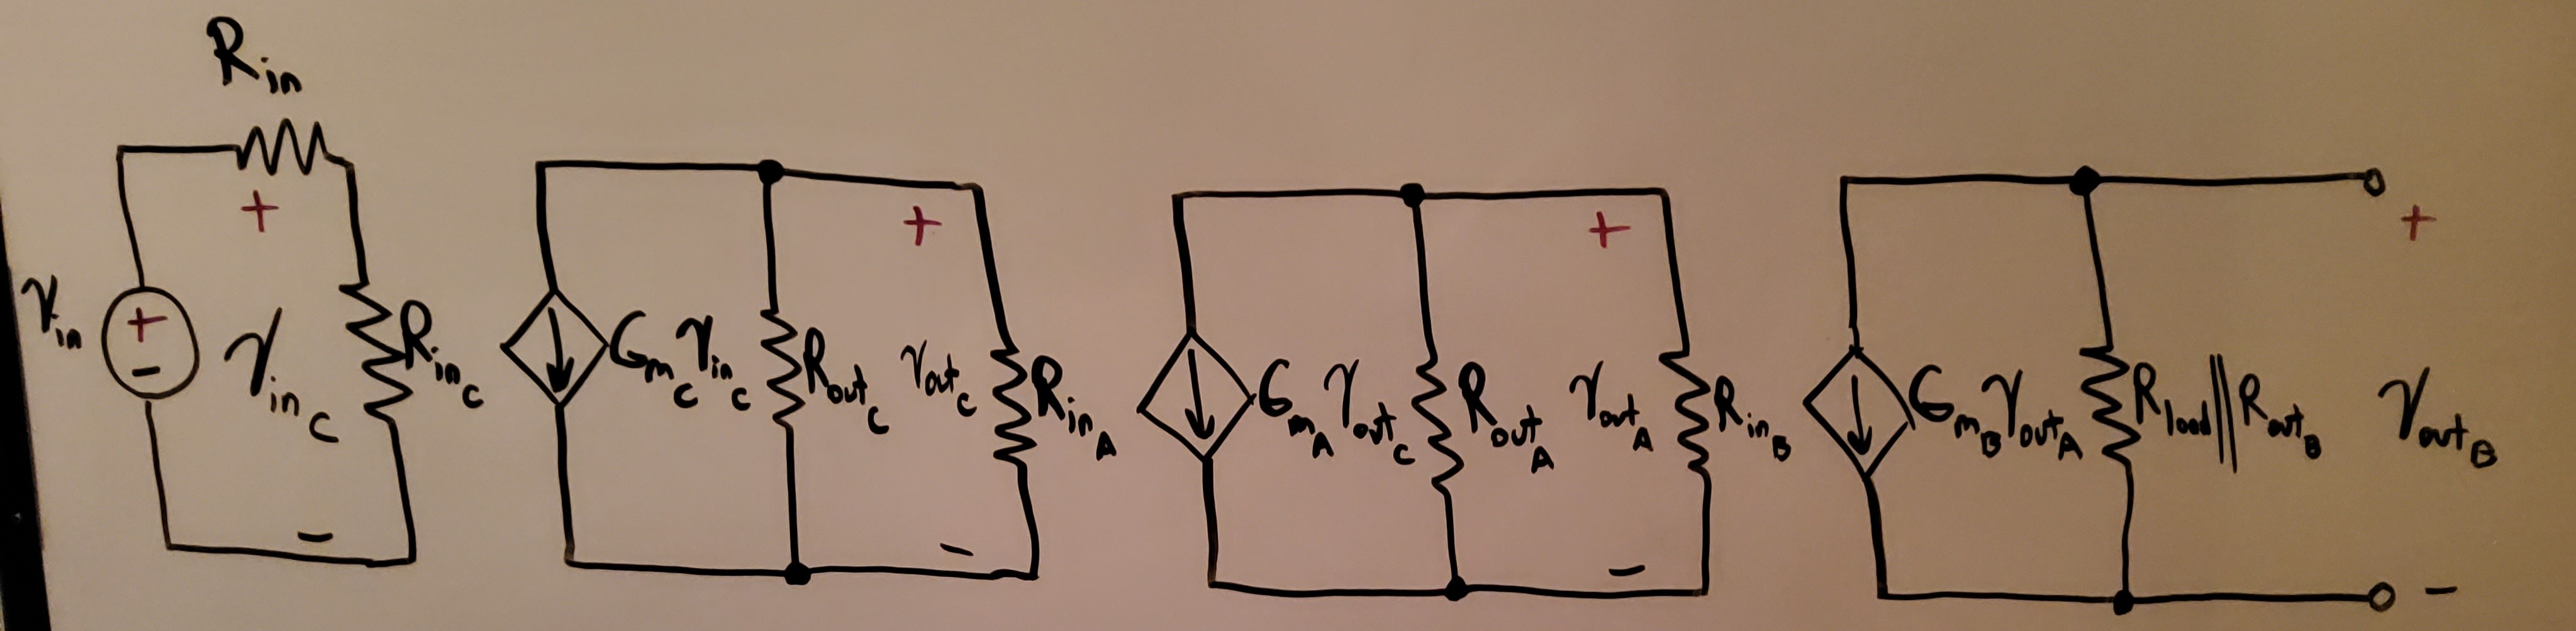
\includegraphics[scale=0.125, center]{p2d.jpg}\\
    
    Note that the subscripts relate to the ordering of the two-port models, where A = part(\textit{a}), B = part(\textit{b}), and C = part(\textit{c}).
    
    \newpage\noindent
    The input current source and resistance are modeled as a Thevenin equivalent ($i_{in} = \frac{v_{in}}{R_{in}}$), and $C_{ac}$ is an AC coupling capacitor, which means that we treat it as a short circuit in this analysis.  Then the overall gain is:
    \begin{equation}
        A_{v_{total}} = \frac{\cancel{v_{{in}_C}}}{v_{in}} \cdot \frac{\bcancel{v_{{out}_C}}}{\cancel{v_{{in}_C}}} \cdot \frac{\cancel{v_{{out}_A}}}{\bcancel{v_{{out}_C}}} \cdot \frac{v_{{out}_B}}{\cancel{v_{{out}_A}}}
        = \frac{v_{{out}_B}}{v_{in}}
    \end{equation}
    We will need to use back-substitution to solve for the overall gain using the $G_m$, $R_{in}$ and $R_{out}$ values already solved for.  We now define all of the voltages in the above equation as they relate to our 2-port models.
    \begin{align*}
        v_{{in}_C} &= v_{in} \left(\frac{R_{{in}_C}}{R_{in} + R_{{in}_C}}\right)\\[0.25cm]
        v_{{out}_C} &= -G_{m_C} v_{{in}_C}(R_{{out}_C} \parallel R_{{in}_A})\\[0.25cm]
        v_{{out}_A} &= -G_{m_A} v_{{out}_C}(R_{{out}_A} \parallel R_{{in}_B})\\[0.25cm]
        v_{{out}_B} &= -G_{m_B} v_{{out}_A}(R_{load} \parallel R_{{out}_B})
    \end{align*}
    
    Then we have:
    \begin{align*}
        A_{v_{total}} &= \frac{v_{{out}_B}}{v_{in}}\\[0.25cm]
        &= \frac{G_{m_B} v_{{out}_A}(R_{load} \parallel R_{{out}_B})}{v_{in}}\\[0.25cm]
        &= \frac{G_{m_B} -G_{m_A} v_{{out}_C}(R_{{out}_A} \parallel R_{{in}_B})(R_{load} \parallel R_{{out}_B})}{v_{in}}\\[0.25cm]
        &= \frac{G_{m_B} G_{m_A} G_{m_C} v_{{in}_C}(R_{{out}_C} \parallel R_{{in}_A})(R_{{out}_A} \parallel R_{{in}_B})(R_{load} \parallel R_{{out}_B})}{v_{in}}\\[0.25cm]
        &= \frac{G_{m_B} -G_{m_A} G_{m_C} \cancel{v_{in}} \left(\frac{R_{{in}_C}}{R_{in} + R_{{in}_C}}\right)(R_{{out}_C} \parallel \cancelto{\infty}{R_{{in}_A}})(R_{{out}_A} \parallel \cancelto{\infty}{R_{{in}_B}})(R_{load} \parallel R_{{out}_B})}{\cancel{v_{in}}}\\[0.25cm]
        \implies \frac{v_{out}}{i_{in} \cdot R_{in}} &= -\left[G_{m_B} G_{m_A} G_{m_C} R_{{out}_C} R_{{out}_A} (R_{load} \parallel R_{{out}_B}) \left(\frac{R_{{in}_C}}{R_{in} + R_{{in}_C}}\right)\right]
    \end{align*}
    }
    Our final expression for the overall gain:
    \begin{equation}
        \boxed{A_{v_{total}} = -\left[G_{m_B} G_{m_A} G_{m_C} R_{{out}_C} R_{{out}_A} (R_{load} \parallel R_{{out}_B}) \left(R_{{in}_C} \parallel R_{in}\right)\right]}
    \end{equation}
\end{enumerate}
\newpage
%%%%%%%%%%%%%%%%%%%%%%%%%%%%%%%%%%%%%%%%%%%%%%%%%%%%%%%%%%%%%%%%%%%%%%%%%%%%%%%%%%%%%%%%%%%%%%%%%%%%%%%%%%%
%                                             APPENDIX                                                    %
%%%%%%%%%%%%%%%%%%%%%%%%%%%%%%%%%%%%%%%%%%%%%%%%%%%%%%%%%%%%%%%%%%%%%%%%%%%%%%%%%%%%%%%%%%%%%%%%%%%%%%%%%%%
\appendix
%%%%%%%%%%%%%%%%%%%%%%%%%%%%%%%%%%%%%%%%%%%%%%%%%%%%%%%%%%%%%%%%%%%%%%%%%%%%%%%%%%%%%%%%%%%%%%%%%%%%%%%%%%%
%                                APPENDIX A: GLOSSARY OF EQUATIONS                                        %
%%%%%%%%%%%%%%%%%%%%%%%%%%%%%%%%%%%%%%%%%%%%%%%%%%%%%%%%%%%%%%%%%%%%%%%%%%%%%%%%%%%%%%%%%%%%%%%%%%%%%%%%%%%
\newpage
\section{Appendix: Glossary of Equations}
    \begin{flalign}
        &&\Aboxed{\phi_{bi} &= \frac{kT}{q} \cdot ln\;\bigg( \frac{N_D \cdot N_A}{{n_i}^2} \bigg)}
        &&\textit{Built-in potential, $PN$-junction}
        \label{eq:phi_bi}
    \end{flalign}

    \begin{flalign}
        &&\Aboxed{W_{dep} &= \sqrt{\frac{2\epsilon_s \left(\phi_{bi} - V_{applied}\right)}{q}
                        \cdot \Bigg( \frac{1}{N_A} + \frac{1}{N_D} \Bigg)}}
        &&\textit{Depletion region width, total}
        \label{eq:total_dep}
    \end{flalign}        

    \begin{flalign}
        &&\Aboxed{C_{dep} &= A \left(\frac{\epsilon_s}{W_{dep}}\right)}
        &&\textit{Junction capacitance}
        \label{eq:junc_cap}
    \end{flalign}

    \begin{flalign}
        &&\Aboxed{I_{DS,sat} &= \left(\frac{W}{2L}\right) \mu_n\,C_{ox}
                         {\big(V_{GS} - V_{T_n}\big)}^2 (1 + \lambda V_{DS})}
        &&\textit{$NMOS$ saturation current}
        \label{eq:mosfet_ids_nmos_sat}\\[0.25cm]
        &&\Aboxed{I_{DS,tri} &= \left(\frac{W}{L}\right) \mu_n\,C_{ox}
                            \left(V_{GS} - V_{T_n} - \frac{V_{DS}}{2}\right) V_{DS}}
        &&\textit{$NMOS$ triode current}
        \label{eq:mosfet_ids_nmos_tri}\\[0.25cm]
        &&\Aboxed{I_{SD,sat} &= \left(\frac{W}{2L}\right) \mu_p\,C_{ox}
                         {\big(V_{SG} - \left|V_{T_p}\right|\big)}^2 (1 + \lambda V_{SD})}
        &&\textit{$PMOS$ saturation current}
        \label{eq:mosfet_ids_pmos_sat}\\[0.25cm]
        &&\Aboxed{I_{SD,tri} &= \left(\frac{W}{L}\right) \mu_p\,C_{ox}
                            \left(V_{SG} - \left|V_{T_p}\right| - \frac{V_{SD}}{2}\right) V_{SD}}
        &&\textit{$PMOS$ triode current}
        \label{eq:mosfet_ids_pmos_tri}
    \end{flalign}

    \begin{flalign}
        &&\Aboxed{r_o &= \frac{1}{\frac{W\,\mu\,C_{ox}}{2L}{(V_{GS} - V_T)}^2\,\lambda}
        \approx \frac{1}{\lambda\,I_{DS}}}
        &&\textit{Output resistance for MOSFET}
        \label{eq:mos_outresistance}
    \end{flalign}

    \begin{flalign}
        &&\Aboxed{g_m &= \left(\frac{W}{L}\right)\mu\,C_{ox}(V_{{DS}_{sat}})
        = \sqrt{\left(\frac{2W}{L}\right)\mu\,C_{ox} I_{DS}}
        = \frac{2 \cdot I_{DS}}{V_{GS} - V_T}}
        &&\textit{Transconductance for MOSFET}
        \label{eq:mos_transconductance}
    \end{flalign}

    \begin{flalign}
        &&\Aboxed{V_{GS} = V_T + \sqrt{\frac{2\,I_{DS}}{\frac{W}{L} \mu C_{ox}}} = V_T + V_{OD}}
        &&\textit{Gate-source condition, diode-connected MOSFET}
        \label{eq:mos_gate_cond}
    \end{flalign}
%%%%%%%%%%%%%%%%%%%%%%%%%%%%%%%%%%%%%%%%%%%%%%%%%%%%%%%%%%%%%%%%%%%%%%%%%%%%%%%%%%%%%%%%%%%%%%%%%%%%%%%%%%%
%                                APPENDIX B: GLOSSARY OF TABLES                                           %
%%%%%%%%%%%%%%%%%%%%%%%%%%%%%%%%%%%%%%%%%%%%%%%%%%%%%%%%%%%%%%%%%%%%%%%%%%%%%%%%%%%%%%%%%%%%%%%%%%%%%%%%%%%
\newpage
\section{Appendix: Glossary of Tables}
    \begin{table}[H]
    \centering
    \setlength{\tabcolsep}{20pt}
    \renewcommand{\arraystretch}{1.5}
    \begin{tabular}{|l|c|c|c|}
        \hline
        \textbf{Transistor Type}  &  \textbf{Cut-off} & \textbf{Triode} & \textbf{Saturation}\\
        \hline
        \textit{NMOS} & $V_{GS} \leq V_{T_n}$
                        & $V_{DS} \leq V_{GS} - V_{T_n}$
                        & $V_{DS} > V_{GS} - V_{T_n}$\\
        \hline
        \textit{PMOS} & $V_{SG} \leq \left|V_{T_p}\right|$
                        & $V_{SD} \leq V_{SG} - \left|V_{T_p}\right|$
                        & $V_{SD} > V_{SG} - \left|V_{T_p}\right|$\\
        \hline
    \end{tabular}
    \caption{Conditions for MOSFET regions of operation.
    \label{tab:mosfet_op}} 
    \end{table}

    \begin{table}[H]
    \centering
    \setlength{\tabcolsep}{20pt}
    \renewcommand{\arraystretch}{1.5}
    \begin{tabular}{|l|c|c|}
        \hline
        \textbf{Description}  &  \textbf{Symbol} & \textbf{Value}\\
        \hline
        Elementary charge & $q$ & $\num{1.60218e-19}\,C$\\
        \hline
        Electron volt & $eV$ & $\num{1.60218e-19}\,J$\\
        \hline
        Boltzmann's constant & $k$ & $\num{1.38066e-23}\,J/K$\\
        \hline
        Free electron mass & $m_0$ & $\num{9.1095e-31}\,kg$\\
        \hline
        Permittivity in vacuum & $\epsilon_0$ & $\num{8.85418e-12}\,F/m$\\
        \hline
        Planck's constant & $h$ & $\num{6.62617e-34}\,J \cdot s$\\
        \hline
        Reduced Planck's constant ($h/2\pi$) & $\hbar$ & $\num{1.05458e-34}\,J \cdot s$\\
        \hline
        Speed of light in vacuum & $c$ & $\num{2.99792e8}\,m/s$\\
        \hline
        Thermal voltage at $T=300^{\circ}K$ & $kT/q$ & $0.0259\,V$\\
        \hline
        Wavelength of 1-$eV$ photon & $\lambda$ & $1.23977\,\mu m$\\
        \hline
    \end{tabular}
    \caption{Physical constants.
    \label{tab:phys_const}} 
    \end{table}
\newpage
    \begin{table}[H]
    \centering
    \setlength{\tabcolsep}{20pt}
    \renewcommand{\arraystretch}{1.5}
    \begin{tabular}{|l|c|c|}
        \hline
        \textbf{Quantity}  &  \textbf{Symbol} & \textbf{Value/Dimension}\\
        \hline
        Meter & $m$ & $1\,m = 10^2\,cm$\\
        \hline
        Millimeter & $mm$ & $1\,mm = 10^{-1}\,cm = 10^{-3}\,m$\\
        \hline
        Micrometer, micron & $\mu m$ & $1\,\mu m = 10^4\,\text{\AA} = 10^3\,mm = 10^{-4}\,cm$\\
        \hline
        Nanometer & $nm$ & $1\,nm = 10\,\text{\AA} = 10^{-3}\,\mu m = 10^{-7}\,cm$\\
        \hline
        Angstrom & $\text{\AA}$ & $1\,\text{\AA} = 10^{-4}\,\mu m = 10^{-8}\,cm = 10^{-10}\,m$\\
        \hline
        Electron volt & $eV$ & $1\,eV = \num{1.60218e-19}\,J$\\
        \hline
        Electric charge (Coulomb) & $C$ & $A \cdot s$\\
        \hline
        Current (Ampere) & $A$ & $C/s$\\
        \hline
        Frequency (Hertz) & $Hz$ & $1/s$\\
        \hline
        Energy (Joule) & $J$ & $N \cdot m$\\
        \hline
        Power (Watt) & $W$ & $J/s$\\
        \hline
        Potential (Volt) & $V$ & $J/C$\\
        \hline
        Conductance (Siemens) & $S$ & $A/V$\\
        \hline
        Resistance (Ohm) & $\Omega$ & $V/A$\\
        \hline
        Capacitance (Farad) & $F$ & $C/V$\\
        \hline
    \end{tabular}
    \caption{Unit conversions.
    \label{tab:unit_conv}} 
    \end{table}
\newpage
%%%%%%%%%%%%%%%%%%%%%%%%%%%%%%%%%%%%%%%%%%%%%%%%%%%%%%%%%%%%%%%%%%%%%%%%%%%%%%%%%%%%%%%%%%%%%%%%%%%%%%%%%%%
%                                           BIBLIOGRAPHY                                                  %
%%%%%%%%%%%%%%%%%%%%%%%%%%%%%%%%%%%%%%%%%%%%%%%%%%%%%%%%%%%%%%%%%%%%%%%%%%%%%%%%%%%%%%%%%%%%%%%%%%%%%%%%%%%
\newpage
\addcontentsline{toc}{section}{References}
\emergencystretch=2em
\nocite{*}
\printbibliography
%%%%%%%%%%%%%%%%%%%%%%%%%%%%%%%%%%%%%%%%%%%%%%%%%%%%%%%%%%%%%%%%%%%%%%%%%%%%%%%%%%%%%%%%%%%%%%%%%%%%%%%%%%%
%                                           END OF DOCUMENT                                               %
%%%%%%%%%%%%%%%%%%%%%%%%%%%%%%%%%%%%%%%%%%%%%%%%%%%%%%%%%%%%%%%%%%%%%%%%%%%%%%%%%%%%%%%%%%%%%%%%%%%%%%%%%%%
\end{document}
